\documentclass[12pt,twoside]{report}
\usepackage[utf8]{inputenc}
\usepackage[a4paper,width=150mm,top=25mm,bottom=25mm,bindingoffset=6mm]{geometry}
\usepackage{graphicx}
\graphicspath{ {images/} }
\usepackage{color}
\usepackage{hyperref}
\hypersetup{
    colorlinks,
    citecolor=black,
    filecolor=black,
    linkcolor=black,
    urlcolor=black
}
\usepackage[style=numeric-comp, sorting=none]{biblatex}
\bibliography{xampl}
\addbibresource{references.bib}
\usepackage{notoccite}
\usepackage{amssymb}
\usepackage{amsmath}
\usepackage{float}
\usepackage{algorithm}
\usepackage{algpseudocode}
\usepackage{listings}
\usepackage[T1]{fontenc}
\usepackage{sourcecodepro}
\lstset{basicstyle=\small\ttfamily}

\title{
    {Phase Transition Continuity Dependence on Edge Evaluation and Acceptance}\\
    {\large Universität Leipzig}
    }
\author{Cameron Perot}
\date{September 2019}


\begin{document}
\maketitle
\pagenumbering{roman}

\chapter*{Abstract}
In 2000 Dmitris Achlioptas asked a question about whether or not there existed processes in which adding edges to a random network would produce a phase transition later than that seen in the traditional Erdős-Rényi model.
Little did he know that this question would have a simple yet complicated answer.
Yes, there did exist such processes and yes they were able to show transitions later than that in the Erdős-Rényi model; however, the continuity of these transitions was not immediately clear.
These processes in question were designed in such a way as to minimize the size of the largest cluster, and in doing so some of them delayed the phase transition to a later point at which it appeared to transition rapidly to the state of large scale connectivity, so rapid that it was brought into question whether the transition was discontinuous.
Over the years there was a lot of research into this topic, eventually concluding that algorithms which take only local information into account produce continuous transitions whereas algorithms that make use of global information can produce discontinuous transitions.
In this thesis we set out to summarize how the field developed as well as produce a new model which exhibits this rapid phase transition behavior.
The new model explored here is called stochastic edge acceptance (SEA), and is a local information based algorithm that uses probabilities (favoring the minimization of the largest cluster) and random numbers to determine which edges to accept.
Analysis of the SEA model performed here shows that it exhibits beautiful power law scaling behavior near the critical point, allowing us to determine critical exponents and show that it does indeed produce a continuous transition.


\tableofcontents
\cleardoublepage
\pagenumbering{arabic}

\chapter{Introduction}
\label{ch:introduction}
%---------------------------------------------------------------------------------------
% What is Percolation Theory?
%---------------------------------------------------------------------------------------
\section{What is Percolation Theory?}
Nature is full of graph-like structures which can be anything from a random network composed of nodes and undirected edges between them to a set of nodes in a periodic arrangement (i.e. a lattice).
To study such structures we need a framework in which to do so; this is where percolation theory enters the picture.
Percolation theory is in the intersection of multiple other topics such as graph theory, probability theory, and statistical physics, combining them in a way to give us the tools we need to study how clusters of nodes behave and evolve within graph-like structures.
Percolation can be observed in a variety of places ranging from the spread of a forest fire to the dissemination of information across a communications network.
We often use percolation theory in physics to help us model how something dissipates or flows through a system, e.g. the electrical conductivity or porousness of a material.
Some of the applications outside of physics include testing the durability of a transportation infrastructure or determining to what extent a product or idea might be adopted by society.
Percolation theory is a broad subject with the ability to be applied to problems in many different disciplines \cite{intro_to_percolation_theory} \cite{applications_of_percolation_theory}.

To get a better understanding of what percolation is let's discuss a few examples.
Society is developing faster than ever before due to the propagation of information and goods through networks we have constructed.
These networks then allow us to create and participate in increasingly more advanced networks, thus it is critical we study and understand how these networks behave so that we can better manage and improve them.
The most well known being the internet, which sustains a massive flow of information between billions of people across the globe.
When something is posted online we might ask: how many people will it reach?
To answer this we would start at the source node then see which nodes it could possibly be connected to.
If each person has a probability $p$ of sharing it with another person then we can construct a probabilistic model to determine what the cluster could possibly look like.
If the probability is high then we would expect the size of cluster to be significant when compared to that of the whole network.

Another interesting application is that to the spread of health epidemics across a population.
If there is a virus going around there is an underlying network that can be studied; there is the initial person(s) who contracted the virus and then the people who were contaminated from coming in contact with those infected.
The obvious question is: how much of the population will it affect?
Let's say in a very basic sense that an infected person has a $p$ percent chance of infecting those they come into contact with.
If the virus is treatable and $p$ is low, then we would expect the virus to be eradicated fairly quickly since doctors have the time and ability to treat the outbreak properly.
On the other hand if $p$ is high, say higher than some critical probability $p_c$, then we might expect a different scenario where the virus spreads across the population, i.e. percolates, much like the Ebola epidemic in West Africa during 2013-2016.
Therefore, percolation theory plays a crucial role in helping us answer important questions when it comes to determining how something might propagate.



%---------------------------------------------------------------------------------------
% Phase Transitions
%---------------------------------------------------------------------------------------
\section{Phase Transitions}
To understand the most important use of percolation theory we must first understand what a phase transition is.
In physics we often encounter systems which have different properties depending on which phase they're in.
Thus we are interested in how the system behaves around the critical point.
A phase transition is usually characterized by an order parameter, which is a variable that is zero in one phase and non-zero in the other; giving us the ability to distinguish phases and identify where the system undergoes transition.

In percolation theory we define the order parameter as the ratio of the largest cluster to the size of the system, i.e. if we have $N$ nodes total and the largest cluster $C$ contains $|C|$ nodes, then the order parameter $m$ is given by:

\begin{equation}
	\label{eqn:order_parameter}
	m := \frac{|C|}{N}
\end{equation}
Of course the system is usually examined in the thermodynamic limit ($N \rightarrow \infty$), this means that $m$ is zero unless there exists a macroscopic cluster.

There are two main types of phase transitions: first- and second-order.
In a first-order phase transition there is what we call a latent heat, i.e. energy that is either absorbed or emitted during a process where the temperature is fixed, e.g. the transition of water between the solid and liquid phases.
Second-order (also called continuous) phase transitions are characterized by a divergent correlation length and power law behavior of variables which leads to a set of critical exponents (more about critical exponents below).
The reason they are called continuous transitions is because the order parameter is continuous at the critical point.
The classic percolation models are known to undergo continuous phase transitions, making them useful for modeling such systems.



%---------------------------------------------------------------------------------------
% Critical Exponents
%---------------------------------------------------------------------------------------
\subsection{Critical Exponents}
Around the critical point in a percolation model there exists a set of numbers called the critical exponents which contain information about how certain quantities of interest behave.
Let's take for example the order parameter as a function of the occupation probability $p$, which is described by the critical exponent $\beta$ \cite{intro_to_percolation_theory}:

\begin{equation}
	\label{eqn:crit_exp_P}
	m(p) \sim (p - p_c)^\beta
\end{equation}
The average cluster size $\langle s \rangle$ is described by $\gamma$ \cite{intro_to_percolation_theory}:

\begin{equation}
	\label{eqn:crit_exp_s}
	\langle s \rangle (p) \sim (p - p_c)^{-\gamma}
\end{equation}
The correlation length $\xi$ is described by $\nu$ \cite{intro_to_percolation_theory}:
\begin{equation}
	\label{eqn:crit_exp_xi}
	\xi (p) \sim |p - p_c|^{-\nu}
\end{equation}

The neat thing about these exponents is that they are universal in the sense that they only depend on the dimension $d$ of the system, regardless of the microscopic configuration.
Some values for these are given in the table below \cite{intro_to_percolation_theory}:

\begin{center}
  \begin{tabular}{ | l | c | c | c | }
    \hline
    $d$ & $\beta$ & $\gamma$ & $\nu$ \\ \hline
    2 & 5/36 & 43/18 & 4/3 \\ \hline
    3 & 0.41 & 1.82 & 0.88 \\
    \hline
  \end{tabular}
\end{center}



%---------------------------------------------------------------------------------------
% Percolation on a Lattice
%---------------------------------------------------------------------------------------
\section{Percolation on a Lattice}
We can look at percolation on a lattice from two different perspectives: site and bond percolation.
With site percolation we study systems where the sites of a lattice are either occupied or unoccupied, whereas with bond percolation we study systems where the edges between sites are either active or inactive.
The underlying concepts of percolation are the same, but in practice the details differ slightly.



\subsection{Site Percolation}
For this we consider a lattice of dimension $d$.
Let's take our lattice to be hyper-cubic with side length $L$, giving us a total of $L^d$ sites in the lattice.
We then occupy each site of the lattice with probability $p$ (unoccupied with probability $1 - p$), independent of all other sites.
We can then use indicator random variables $X_1, ..., X_{L^d}$ to represent if the sites are occupied or not, where:

\[
X_i =
\begin{cases}
	1 & \text{if site } i \text{ occupied} \\
	0 & \text{otherwise}
\end{cases}
\]

The number of occupied sites in the lattice is then given by $\sum_i X_i$, which is expected to be $L^d p$.
The notion of a cluster $I = \{i_1, ..., i_s\}$ of size $s = \sum_{i \in I} X_i$ is defined as a set of $s$ occupied sites which are nearest neighbors with at least one other site in the set.
If we let $N_s$ represent the number of clusters of size $s$, and $n_s = N_s / L^d$, then we can also look at the probability that any given site is part of a cluster:

\begin{equation}
	\label{eqn:p_in_cluster}
	\sum_s s n_s
\end{equation}

This now gives us the ability to determine the probability that the given site is part of a cluster of size $s$:

\begin{equation}
	\label{eqn:p_in_cluster_size_s}
	\frac{s n_s}{\sum_{s'} s' n_s'}
\end{equation}

Using the above we can compute the average cluster size:

\begin{equation}
	\label{eqn:avg_cluster_size}
	\langle s \rangle = \sum_s s \frac{s n_s}{\sum_{s'} s' n_s'}
\end{equation}

Therefore, it is clear that we can obtain a significant amount of information by applying basic probability theory.
Now that we have defined clusters and cluster sizes we can talk about the idea of a percolating cluster.
This is a cluster which spans from one side of the lattice to the opposite in any of the $d$ dimensions.
It's obvious that the presence of a percolating cluster is heavily dependent on $p$, since for low $p$ we wouldn't expect to see a cluster spanning across the lattice.
However, this is also dependent on $L$, and we often seek to study the limiting case where $L \rightarrow \infty$.
This leads us to the concept of a critical probability, $p_c$, such that when $p > p_c$ we expect to see a percolating cluster, but not when $p < p_c$.

\paragraph{One-Dimension}
We now consider the simplest case where $d = 1$, which allows us to analytically solve for some quantities of interest.
Fig. \ref{fig:1d_site_clusters} illustrates a snippet of an infinite 1D lattice where the solid black sites are active and the hollow white ones are inactive.
There are a total of four clusters visible (highlighted in blue): two one-clusters, a three-cluster, and a four-cluster.

\begin{figure}[H]
	\centering
	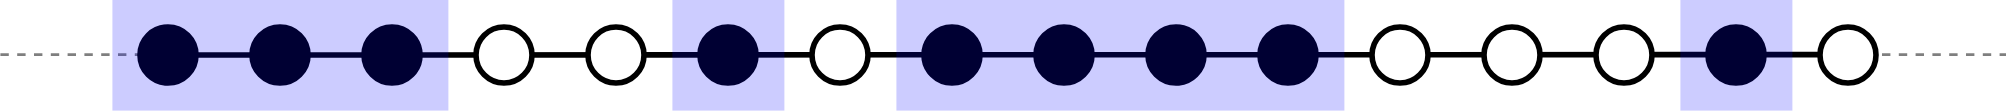
\includegraphics[width=350pt]{images/1d_site_clusters.png}
	\caption{1D Site Clusters}
	\label{fig:1d_site_clusters}
\end{figure}

For comparison Fig. \ref{fig:1d_bond_clusters} illustrates a 1D lattice where all sites are active and only some of the bonds between them are active.
There are a total of four clusters visible (highlighted in blue): two two-clusters, a three-cluster, and a four-cluster.

\begin{figure}[H]
	\centering
	\includegraphics[width=350pt]{images/1d_bond_clusters.png}
	\caption{1D Bond Clusters}
	\label{fig:1d_bond_clusters}
\end{figure}

The probability that any given site is part of a cluster of size $s$ is then given by the product of the independent probabilities of the site to the left of the leftmost site in the cluster being unoccupied, $s$ consecutive sites being occupied, and the site to the right of the rightmost site in the cluster being unoccupied, i.e.:

\begin{equation}
	\label{eqn:n_s_1d}
	n_s = (1 - p) \cdot p^s \cdot (1 - p) = p^s (1 - p)^2
\end{equation}

Plugging Eq. \ref{eqn:n_s_1d} into Eq. \ref{eqn:p_in_cluster} we find:

\begin{equation}
\begin{split}
	\sum_s n_s s &= (1 - p)^2 \sum_s s p^s\\
	&= (1 - p)^2 p \frac{d}{dp} \sum_s p^s\\
	&= (1 - p)^2 p \frac{d}{dp} \frac{p}{1-p}\\
	&= (1 - p)^2 p \bigg[ \frac{1}{1-p} + \frac{p}{(1 - p)^2} \bigg]\\
	&= p
\end{split}
\end{equation}

Where the second equality is obtained by linearity of the derivative and summation operators and realizing that $s p^s = p \frac{d}{dp} p^s$, the third by noticing that $\sum_s p^s$ is the power series for $\frac{p}{1-p}$, the fourth by application of the derivative operator, and the final by algebaic manipulation.
Therefore, there is a $p$ percent chance that any given site is part of a cluster, which when thought about is fairly obvious.
Using the above we can also analytically determine the average cluster size (again using the trick of differentiating $p^s$ to bring down an $s$):

\begin{equation}
\begin{split}
	\langle s \rangle &= \sum_s \frac{s^2 n_s}{\sum_{s'} s' n_s'}\\
	&= \frac{(1 - p)^2}{p} \sum_s s^2 p^s\\
	&= \frac{(1 - p)^2}{p} \bigg[p\frac{d}{dp}\bigg]^2 \sum_s p^s\\
	&= \frac{(1 - p)^2}{p} \bigg[p\frac{d}{dp}\bigg]^2 \frac{p}{1 - p}\\
	&= \frac{(1 - p)^2}{p} p \frac{d}{dp} \bigg[ \frac{p}{1-p} + \frac{p^2}{(1 - p)^2} \bigg]\\
	&= \frac{1 + p}{1 - p}
\end{split}
\end{equation}

The above illustrates that we can analytically solve for some of the quantities of interest in the one-dimensional case.
We're often more interested in the thermodynamic limit, i.e. when $L \rightarrow \infty$.
In the thermodynamic limit percolation on the chain only occurs when we have an infinite number of neighboring occupied sites.
This means that if just one site out of the entire chain is unoccupied there is no percolating cluster which leads us to conclude that for the one-dimensional case $p_c = 1$.

\paragraph{Multiple-Dimensions}
Unfortunately it is not as straight forward in higher dimensions due to the many different arrangements and shapes that the clusters can take on.
This is illustrated in Fig. \ref{fig:2d_site_clusters} where we can see four possible arrangements of a nine-cluster, each with different numbers of neighboring inactive sites.

\begin{figure}
	\centering
	\includegraphics[width=300pt]{images/2d_site_clusters.png}
	\caption{2D Site Clusters}
	\label{fig:2d_site_clusters}
\end{figure}
Without the ability to answer our questions through analytical methods we must resort to numerical methods and simulations to study the system.
This is where computer simulations and finite-size scaling analysis come in handy.
Due to the limitations of computational power we can only simulate systems up to certain sizes; however, we would still like to gather some information about the infinite size system.
What we do is we simulate systems of varying sizes and see how the quantities of interest scale with the system size, which gives us the ability to extrapolate to the thermodynamic limit.

\paragraph{Example: Ising Model}
The Ising model is the most well-known model of ferromagnetism, undergoing a second-order phase transition (for $d \ge 2$) from the ordered, ferromagnetic state at low temperatures to the disordered, paramagnetic state at high temperatures.
This model has played a significant role in the development and understanding of statistical physics.
The basic idea is that given a lattice of size $L^d$, at each site $i$ of the lattice there is a spin $\sigma_i$ oriented in either the up or down direction.
The order parameter characterizing the transition is the magnetization $m = \frac{1}{L^d} \sum_i \sigma_i$.
A (simplified) Hamiltonian of the system in the configuration $\{\sigma\}$ is then given by:

\begin{equation}
	\label{eqn:Ising_Hamiltonian}
	H(\{\sigma\}) = -J \sum_{\langle i j \rangle} \sigma_{ij} -h \sum_i \sigma_i
\end{equation}
Where the sum is over all neighboring spin pairs, $J$ is the coupling constant between spins, and $h$ is a mean field per spin approximation.
Using this combined with statistical and computational physics methods we are able to simulate how this system behaves as the size increases.
One useful tool when modeling such a system is the use of periodic boundary conditions, which help reduce the finite-size effects of smaller lattice sizes.
In Fig. \ref{fig:Ising_percolation} we can see a percolating cluster of up (black) spins at the critical temperature $T_c = 2 / \log(1 + \sqrt{2})$ on a 2D square lattice with side-length $L = 128$.
Fig. \ref{fig:Ising_percolation} was generated using the Wolff single cluster algorithm with $5 \cdot 10^4$ update sweeps over the lattice.

\begin{figure}[H]
	\centering
	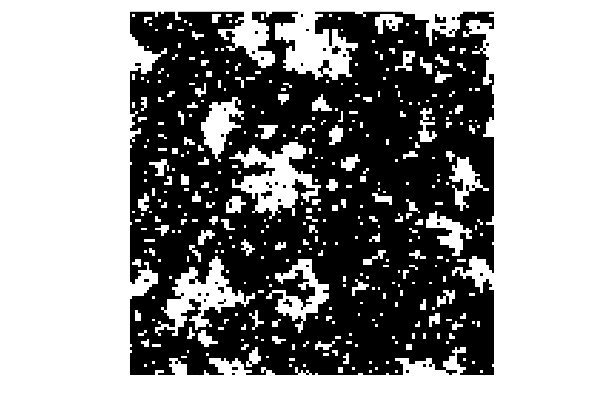
\includegraphics[width=350pt]{images/Ising_128_percolation.png}
	\caption{2D Ising Model Percolating Cluster}
	\label{fig:Ising_percolation}
\end{figure}



%---------------------------------------------------------------------------------------
% Percolation on a Random Network
%---------------------------------------------------------------------------------------
\section{Percolation on a Random Network}
Percolation can also be observed on networks, so we will now discuss some of the basic ideas behind network percolation as a segue to the next section.
In the late 1950s and early 1960s Paul Erdős and Alfréd Rényi published several papers on random networks, leading to the creation of what is known today as the Erdős-Rényi (ER) model \cite{ER_1} \cite{ER_2}.

To get an idea of how it works we imagine a graph starting with a set of $N$ disconnected nodes at $t = 0$, giving us ${N \choose 2}$ possible connections between them.
Then at each step in the evolution process two nodes are chosen at random and connected by an edge, thus after $t$ steps there are a total $t$ edges present in the network.

A cluster on a random network is a set of nodes connected by edges, either directly or indirectly.
Being that some clusters in the graph will of course merge together over time, there exists an attractive potential of sorts between clusters corresponding to the likelihood that the clusters will merge together to form a larger one.
To demonstrate this let's take three clusters $C_1, C_2,$ and $C_3$ of sizes $|C_1|, |C_2|,$ and $|C_3|$, with $|C_1| > |C_2|$ leaving $|C_3|$ arbitrary.
Then we let $\Phi_1$ ($\Phi_2$) be the potential between the first (second) cluster and the third.
In a network where each connection is equally probable, the probability that the first or second cluster merges with the third is directly proportional to the size of the cluster because more nodes means more possible connections.
Therefore, there is a higher probability that the first cluster rather than the second merges with the third and we conclude that $\Phi_1 > \Phi_2$.

Percolation occurs in a network when a giant (macroscopically large) cluster appears.
The order parameter here is defined as the largest cluster size divided by the network size, i.e. $|C| / N$.
Let $N$ be the number of nodes, $t$ be the number of edges present in the graph, and take $r = t/N$.
If $r > 0.5$ then there will exist a percolating cluster within the graph, but not if $r < 0.5$ \cite{ER_2}. This tells us that $r_c = 0.5$ is the critical point where the system transitions from the disconnected state to the state of large scale connectivity.
Letting $|C|$ be the size of the largest cluster, it can be shown that for $r < 0.5$ the largest cluster size scales as $C \sim \log N$, and for $r > 0.5$ $C \sim N$, and more specifically if $r \gtrsim 0.5$ one finds $C \approx (4r - 2)N$ \cite{ER_2}.
This tells us that the ER model exhibits a continuous phase transition when the number of edges exceeds half the number of nodes in the graph.
Looking at Fig. \ref{fig:ER_transition} we can see that the order parameter is zero up until $r = 0.5$ when it transitions to the state of large scale connectivity.

\begin{figure}[H]
	\centering
	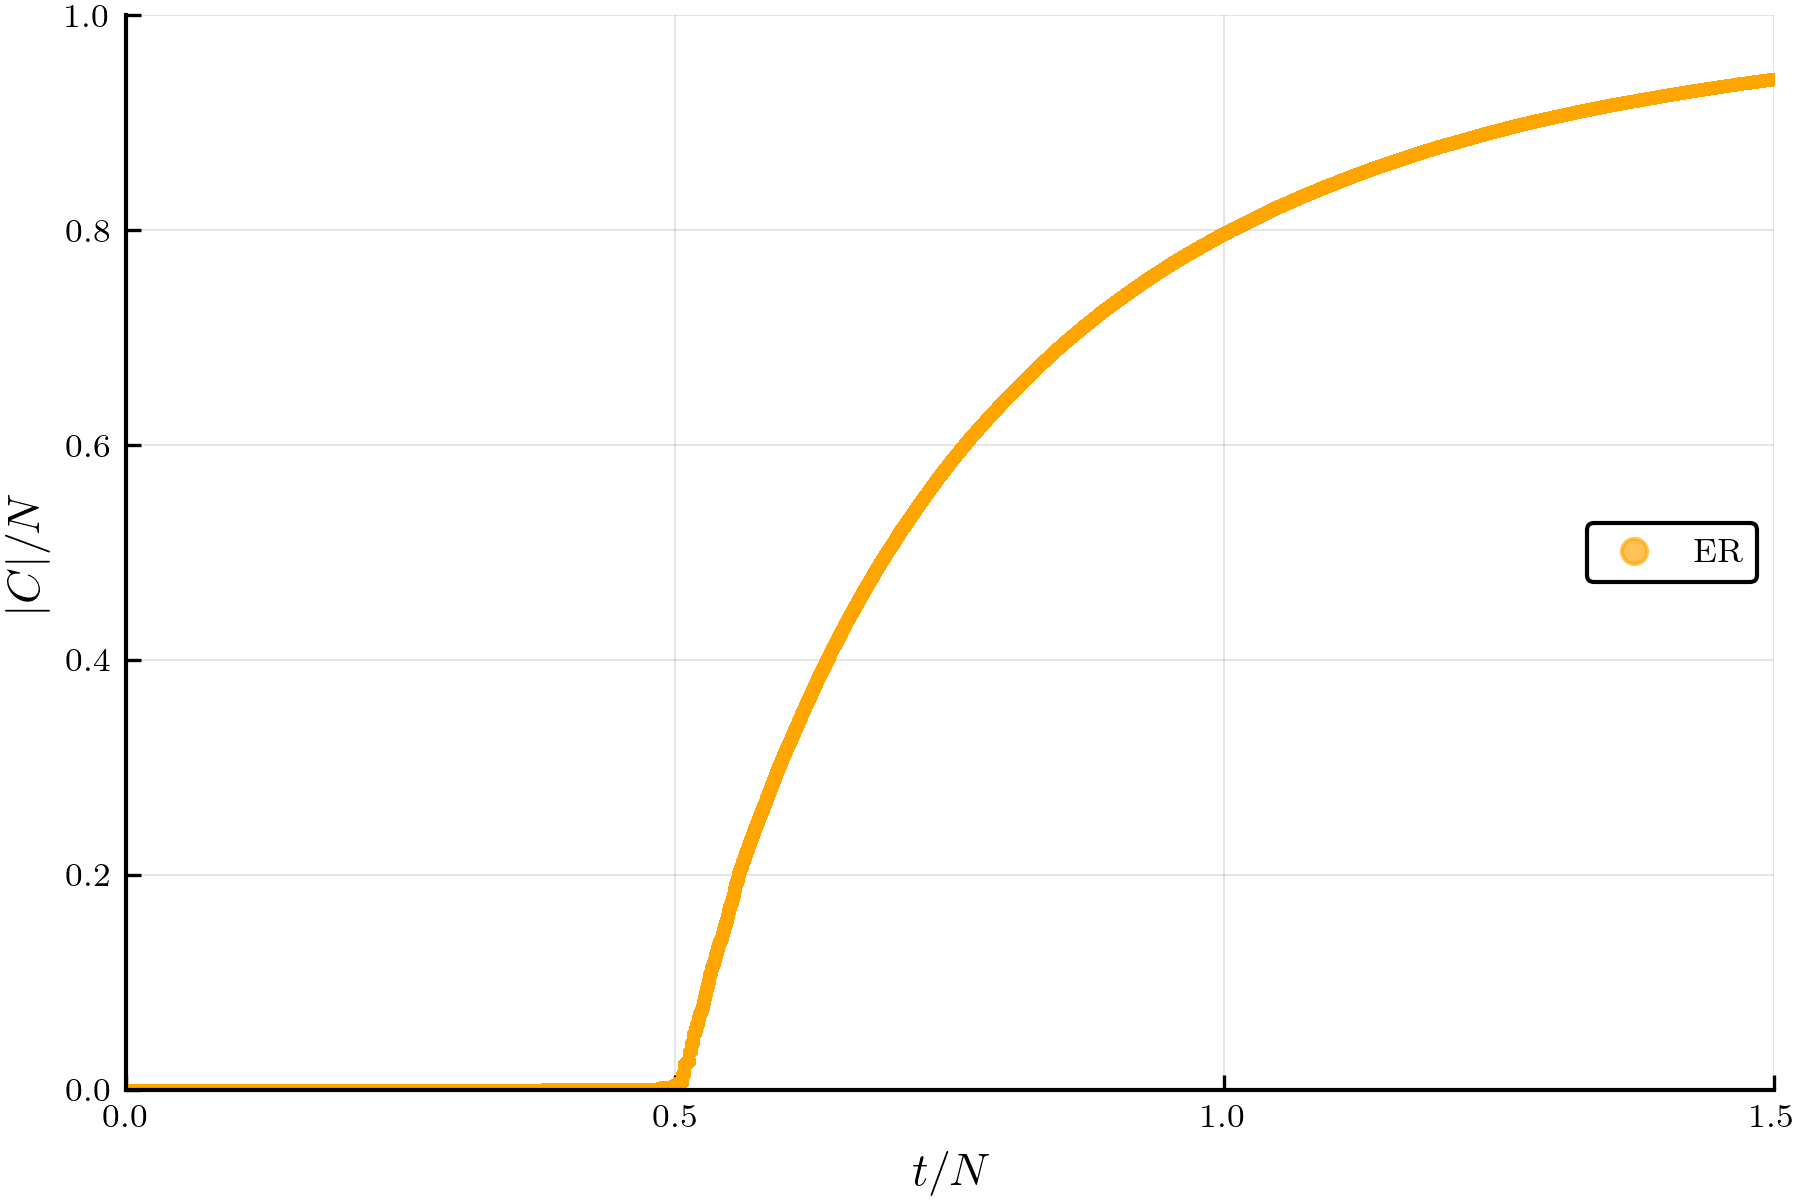
\includegraphics[width=350pt]{images/Network_ER_1e6_order_param.png}
	\caption{Erdős-Rényi model order parameter as a function of the number of edges divided by the system size. It transitions phases right at $r = 0.5$ as has been proven \cite{ER_2}. $N = 10^6$.}
	\label{fig:ER_transition}
\end{figure}


\chapter{An "Explosive" Transition}
\label{ch:explosive}
%---------------------------------------------------------------------------------------
% An Explosive Transition
%---------------------------------------------------------------------------------------
\section{An "Explosive" Transition}
In this paper we are going to take a deeper look into a specific type of percolation referred to as explosive percolation, where the underlying concept is that the onset of percolation is delayed until a certain point where it then occurs at an accelerated rate.
This occurs when the underlying evolution process works in such a way that the largest cluster size $|C|$ is controlled.
We can think of a graph where multiple clusters might evolve separately without merging.
Collectively they take up a large portion of the graph but there isn't a percolating cluster yet due to the lack of connections between the them.
If at some point these clusters do begin to connect then the graph transitions to the percolating state.
For certain evolution processes it has been heavily debated whether or not the phase transition is continuous or not, so the aim of the next section is to summarize what we know to this point regarding the nature of the transition for said processes.



%---------------------------------------------------------------------------------------
% A Selective Process
%---------------------------------------------------------------------------------------
\subsection{A Selective Process}
This all started in the year 2000 when Dimitris Achlioptas raised an interesting question about how a graph of $N$ nodes would evolve under certain conditions \cite{BF}.
First we suppose that at each step $t$ in the evolution process two edges $e_t$ and $e_t'$ are evaluated, but only one of them is chosen to be added to the graph.
Which of the proposed edges is chosen is based only on the information contained in $e_1, e_1', ... e_{t-1}, e_{t-1}'$.
Does there exist an algorithm for adding edges to the graph such that with high probability a giant component does not appear until $t/N > 0.5$?
This process of evaluating $m \ge 2$ edges at each step is now referred to as an $q$-edge Achlioptas process.
In the next few sections we will see how a small change to the way edges are added can have a big impact on the evolution of the system.



%---------------------------------------------------------------------------------------
% The First Look
%---------------------------------------------------------------------------------------
\subsection{The First Look}
In 2001 Tom Bohman and Alan Frieze were the first to design and analyze an Achlioptas process in their paper "Avoiding a Giant Component" \cite{BF}, where they set out to answer Achlioptas' question.
This paper laid out the framework for the Bohman-Frieze (BF) model and showed that there does exist a process in which the appearance of a giant cluster is delayed; so the answer to Achlioptas' question is yes!
This can be seen in Fig. \ref{fig:ER_BF_transition} where the order parameter for the BF model remains smaller than for the ER model, but a little after $r = 0.5$ it begins to rise at a faster rate than in the ER model, eventually overtaking the ER model.

\begin{figure}[H]
	\centering
	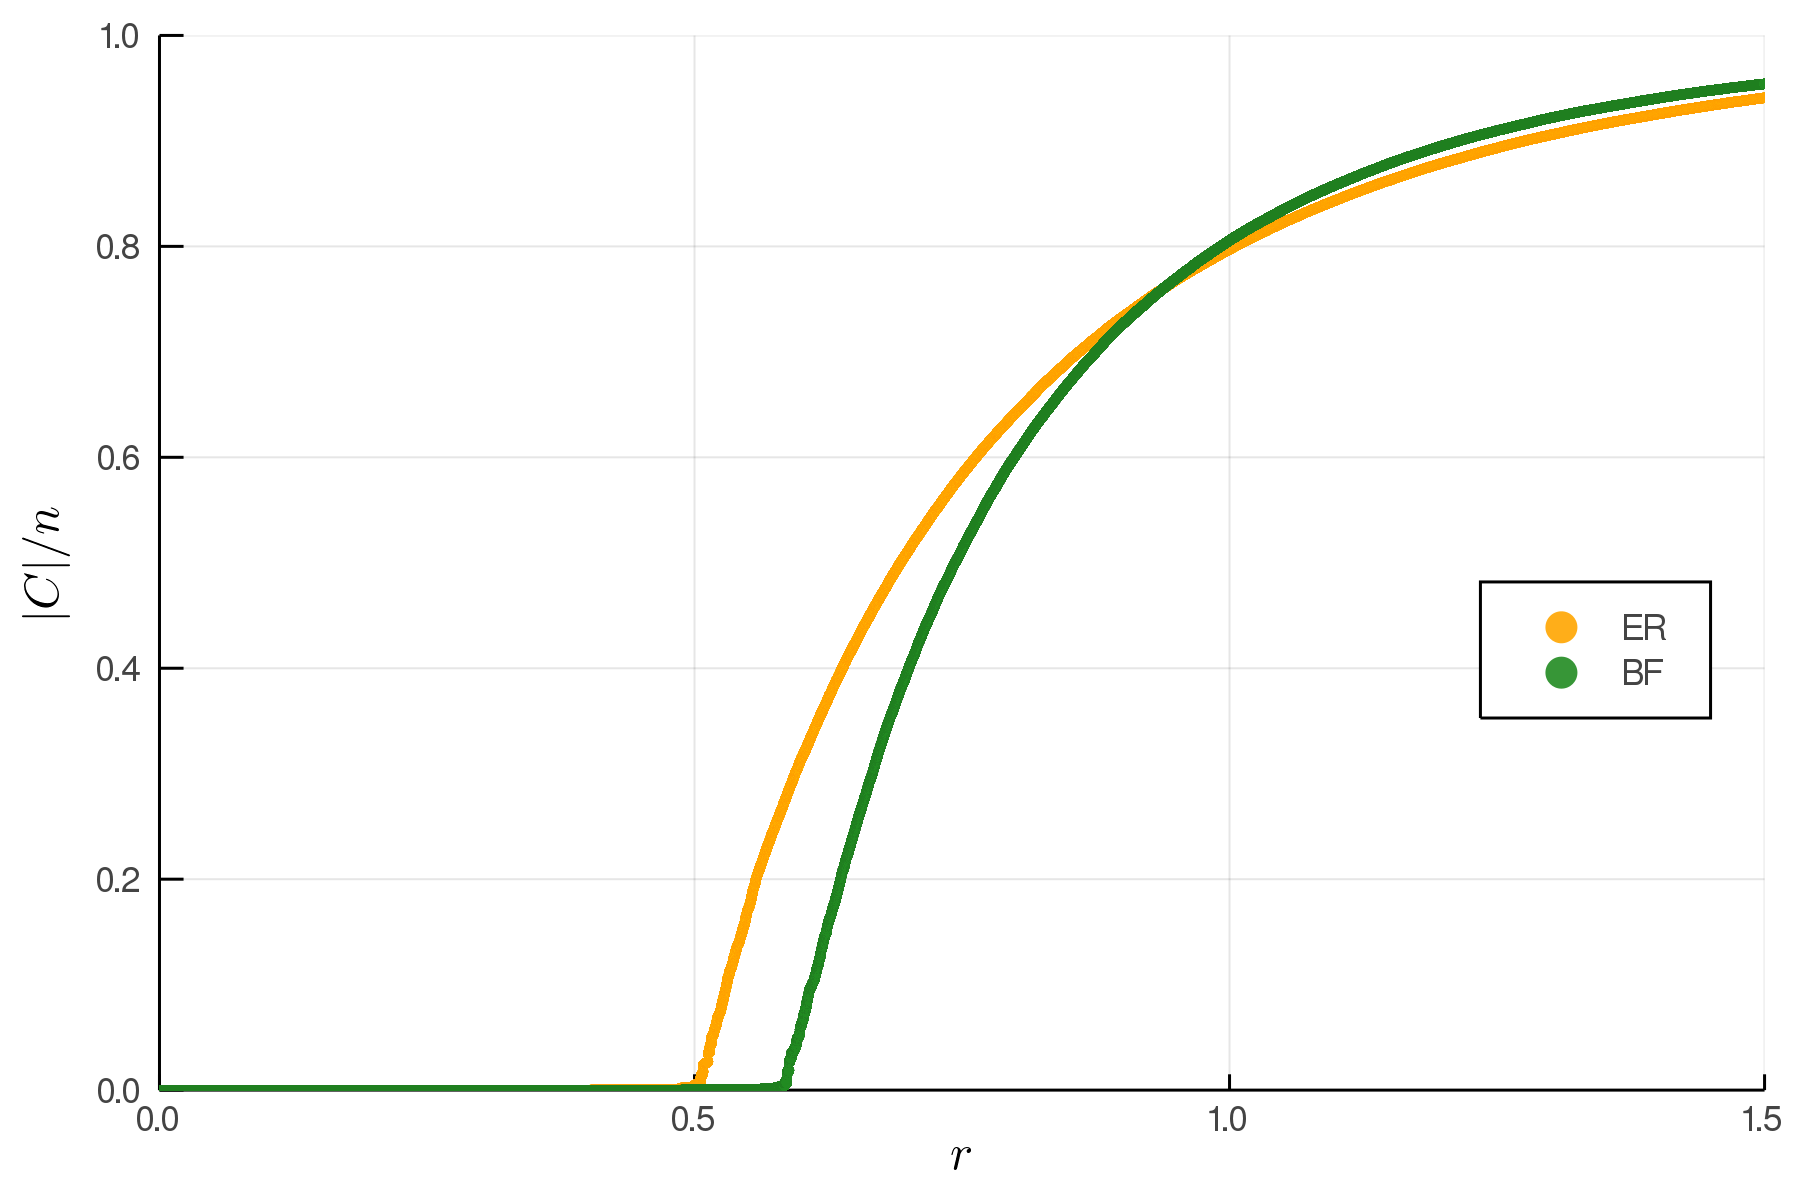
\includegraphics[width=350pt]{images/Network_ER_BF_1e6_order_param.png}
	\caption{Bohman-Frieze model order parameter compared to that of the ER model. It is clear that the transition is delayed to a point beyond 0.5. $N = 10^6$.}
	\label{fig:ER_BF_transition}
\end{figure}

The algorithm they came up with randomly/uniformly samples and evaluates two edges $e_t$ and $e_t'$ at each step $t$, adding $e_t$ if it connects two isolated nodes and discarding $e_t'$, otherwise adding $e_t'$ and discarding $e_t$.
This is known as a bounded-size rule which has since been generalized to a $K$ bounded-size rule where $e_t$ is added if it connects clusters of size smaller than $K$, otherwise $e_t'$ is added.
What this process does is equally discriminate against clusters of size greater than or equal to $K$.
It has been hypothesized that all bounded-size rules exhibit continuous phase transitions \cite{Spencer_Wormald}.

A form of the algorithm can be written in pseudocode as follows:
\begin{itemize}
	\item Let $T$ be the total number of edges to add to the graph.
	\item Let $A_t = \{e_1, e_2, ..., e_t\}$ be the set of accepted edges at step $t$.
	\item Let $e_t^1$ and $e_t^2$ be the two nodes which edge $e_t$ would connect.
	\item Let $C(e_t^i)$ be the cluster which $e_t^i$ belongs to.
\end{itemize}

\begin{algorithm}[H]
	\caption{Bohman-Frieze}\label{Bohman-Frieze}
	\begin{algorithmic}[1]
		\Procedure{BF}{$T, K=2$}
		\State $A \gets \emptyset$
		\State $t \gets 1$
		\While{$t \le T$}
			\If{$|C(e_t^1)| < K$ and $|C(e_t^2)| < K$}
				\State $A \gets A \cup \{e_t\}$
			\Else
				\State $A \gets A \cup \{e_t'\}$
			\EndIf
			\State $t \gets t+1$
		\EndWhile
	\EndProcedure
	\end{algorithmic}
\end{algorithm}

A few years after their original paper, Bohman and Frieze published another paper with Nicholas Wormald titled "Avoidance of a giant component in half the edge set of a random graph" \cite{BFW}.
In this paper they designed a new algorithm (BFW) for adding edges to a graph that runs in phases beginning at $k = 2$.
Starting with $N$ isolated nodes, edges are randomly/uniformly sampled and evaluated one at a time.
If the edge being evaluated would create a cluster of size less than or equal to $k$ then the edge is accepted, otherwise the edge is rejected.
If edge is rejected and the ratio of accepted edges is less than the function $g(k) = 1/2 + \sqrt{1/(2k)}$, then the algorithm moves to the next phase.

A form of the algorithm can be written in pseudocode as follows:
\begin{itemize}
	\item Let $T$ be the total number of edges to add to the graph.
	\item Let $A_i = \{e_1, e_2, ..., e_i\}$ be the set of accepted edges at step $i$.
	\item Let $C(A)$ be the largest cluster in $A$.
\end{itemize}

\begin{algorithm}[H]
	\caption{Bohman-Frieze-Wormald}\label{Bohman-Frieze-Wormald}
	\begin{algorithmic}[1]
		\Procedure{BFW}{$T$}
		\State $A \gets \emptyset$
		\State $k \gets 2$
		\State $t \gets 1$
		\State $i \gets 1$

		\While{$t \le T$}
			\If{$|C(A \cup \{e_i\})| \le k$}
				\State $A \gets A \cup \{e_i\}$
				\State $t \gets t+1$
				\State $i \gets i+1$
			\ElsIf{$|A|/i < g(k)$}
				\State $k \gets k+1$
			\Else
				\State $i \gets i+1$
			\EndIf
		\EndWhile
	\EndProcedure
	\end{algorithmic}
\end{algorithm}



%---------------------------------------------------------------------------------------
% A Discontinuous Transition
%---------------------------------------------------------------------------------------
\subsection{A Discontinuous Transition?}
The first mention of explosive percolation appeared in 2009 in the paper "Explosive Percolation in Random Networks" \cite{Achlioptas_1} by Dimitris Achlioptas, Raissa M. D’Souza, and Joel Spencer, which will henceforth be referred to as Achlioptas et al.
In this paper they laid out a method of evaluating candidate edges called the product rule (PR).
At each step $t$ in the evolution process two edges are selected randomly/uniformly and evaluated based on the product of the cluster sizes that the edges would connect.
More specifically, if edge $e_t$ connects clusters $C(e_t^1)$ and $C(e_t^2)$ and edge $e_t'$ connects clusters $C(e_t'^1)$ and $C(e_t'^2)$, then $e_t$ is accepted if $|C(e_t^1)| \cdot |C(e_t^2)| < |C(e_t'^1)| \cdot |C(e_t'^2)|$, otherwise $e_t'$ is accepted.

A form of the algorithm can be written in pseudocode as follows:
\begin{itemize}
	\item Let $T$ be the total number of edges to add to the graph.
	\item Let $A_t = \{e_1, e_2, ..., e_t\}$ be the set of accepted edges at step $t$.
	\item Let $e_t^1$ and $e_t^2$ be the two nodes which edge $e_t$ would connect.
	\item Let $C(e_t^i)$ be the cluster which $e_t^i$ belongs to.
\end{itemize}

\begin{algorithm}
	\caption{Product Rule}\label{Product-Rule}
	\begin{algorithmic}[1]
		\Procedure{PR}{$T$}
		\State $A \gets \emptyset$
		\State $t \gets 1$

		\While{$t \le T$}
			\If{$|C(e_t^1)| \cdot |C(e_t^2)| < |C(e_t'^1)| \cdot |C(e_t'^2)|$}
				\State $A \gets A \cup \{e_t\}$
				\State $t \gets t+1$
			\Else
				\State $A \gets A \cup \{e_t'\}$
				\State $t \gets t+1$
			\EndIf
		\EndWhile
	\EndProcedure
	\end{algorithmic}
\end{algorithm}

This is illustrated in Fig. \ref{fig:edge_selection} where the first proposed edge $e_t$ would connect the blue cluster of size 5 to the red cluster of size 3 and the second proposed edge $e_t'$ would connect the orange cluster of size 2 to the green cluster of size 4.
The product corresponding to $e_t$ is $5 \cdot 3 = 15$ whereas the product corresponding to $e_t'$ is $2 \cdot 4 = 8$, so $e_t$ is rejected and $e_t'$ accepted.
If we were looking at Fig. \ref{fig:edge_selection} from within the framework of the BF model with $K = 1$, then $e_t$ would be rejected and $e_t'$ accepted even though both the orange and green clusters are of size greater than $K$.

\begin{figure}[H]
	\centering
	\includegraphics[width=200pt, clip]{images/edge_selection.png}
	\caption{Edge Selection}
	\label{fig:edge_selection}
\end{figure}

Fig. \ref{fig:ER_BF_PR_transition} shows the order parameters for the ER, BF, and PR models, making it clear just how drastically different the PR model transition is than in the other models.
As can be seen the order parameter remains near zero for much longer until the critical point $r_c \approx 0.888...$, which is much later than the critical point in the ER model of $r_c = 0.5$.
Not long after the critical point is reached the order parameter appears to jump up discontinuously, which was a surprising find.

\begin{figure}[H]
	\centering
	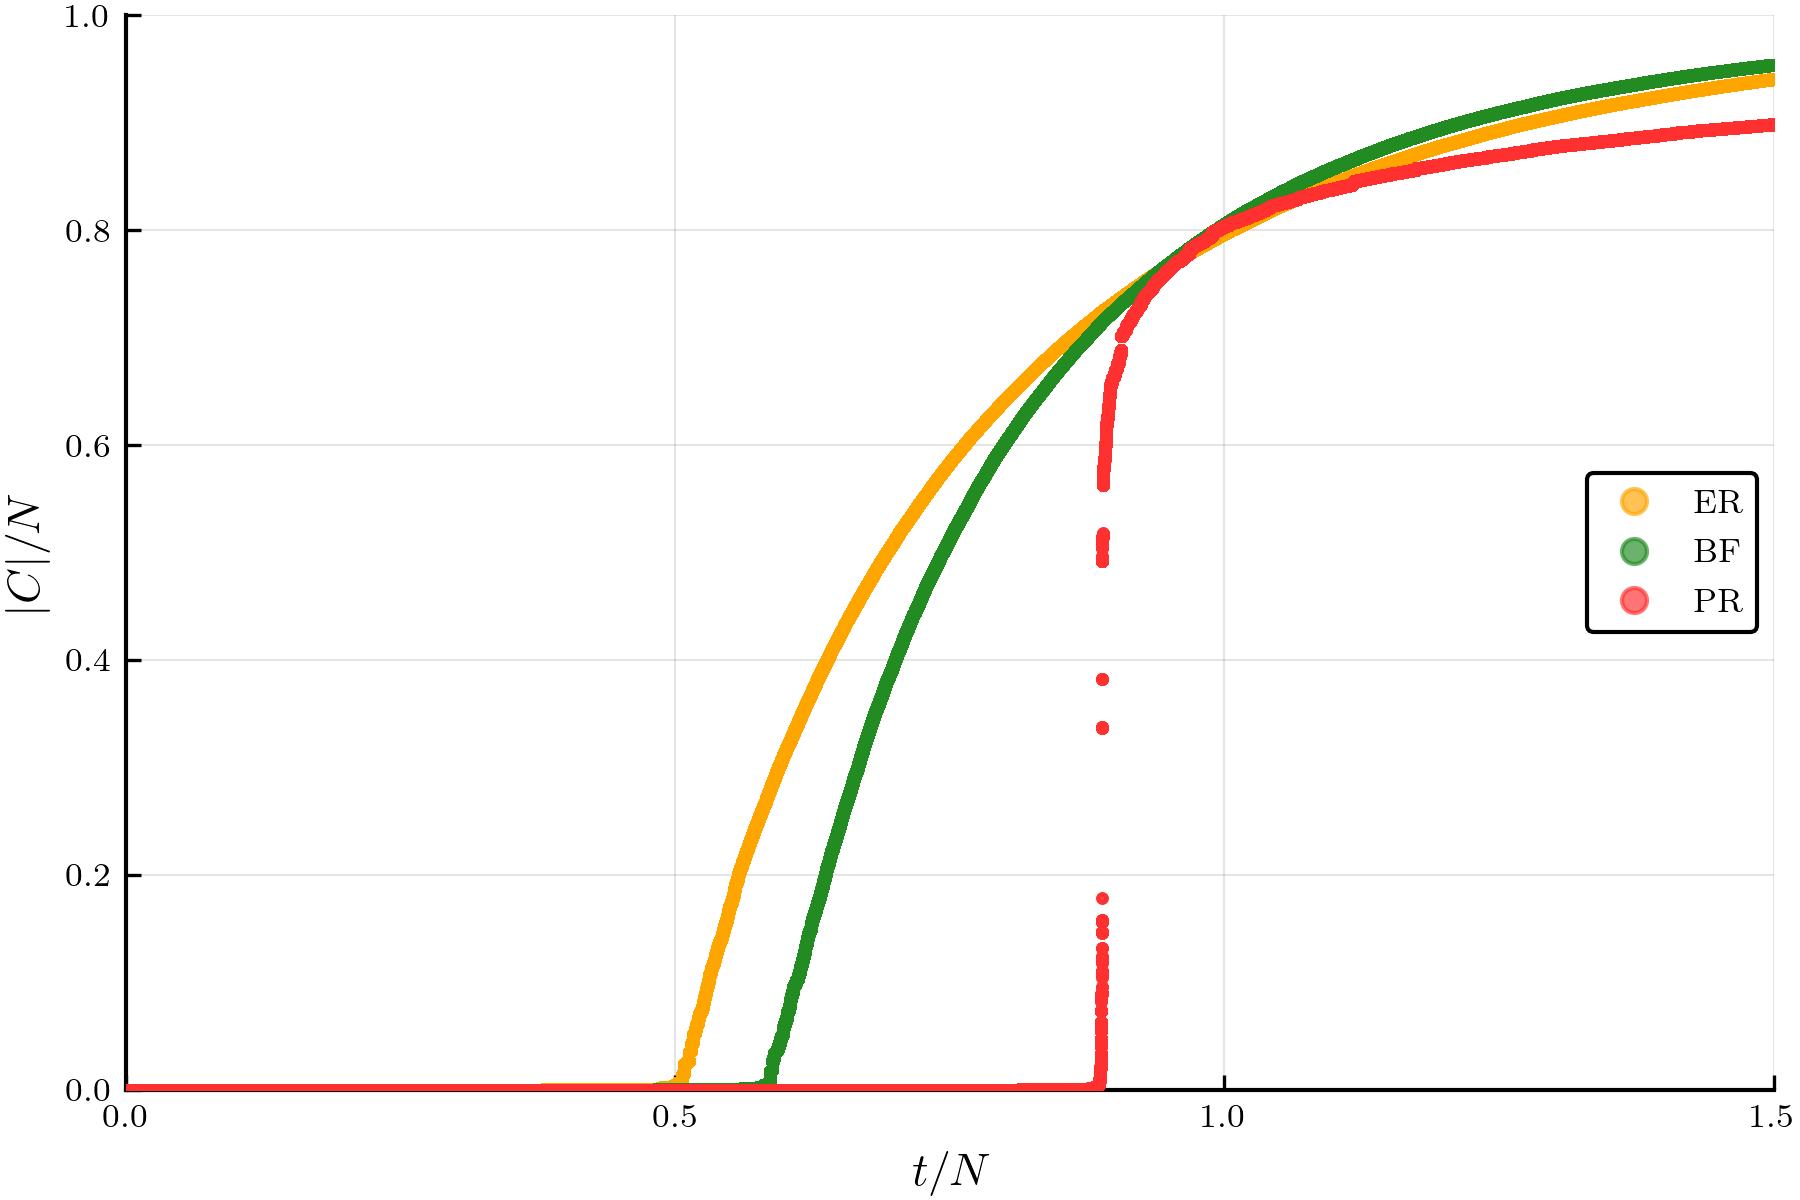
\includegraphics[width=350pt]{images/Network_ER_BF_PR_1e6_order_param.png}
	\caption{Product rule model order parameter plotted with the ER and BF models for comparison. The transition is much more delayed than that of BF, and has an almost vertical slope to the order parameter at the critical point. $N = 10^6$.}
	\label{fig:ER_BF_PR_transition}
\end{figure}

In their paper they analyzed the scaling behavior of their model, defining the quantity $\Delta := t_1 - t_0$, where $t_0$ is the last step where $C < N^{1/2}$ and $t_1$ is the first step where $C > 0.5N$.
$\Delta$ is linear in $N$ for continuous transitions (i.e. an extensive quantity), however, their analysis indicated otherwise that $\Delta < 2N^{2/3}$ and $\Delta / N^{2/3} \rightarrow 1$ in their simulations for sizes up to $6.4 \cdot 10^7$.
To arrive at these results they took an ensemble average of 50 different independent and identically distributed observations and fit a curve to determine the relation between $\Delta$ and $N$.
Their findings are illustrated in Fig. \ref{fig:achlioptas_plots}.

\begin{figure}[H]
	\centering
	\includegraphics[width=400pt]{images/achlioptas_plots.png}
	\caption{Achlioptas et al. simulation results. Source: \cite{Achlioptas_1}.}
	\label{fig:achlioptas_plots}
\end{figure}

They ended their paper by saying: "We have demonstrated that small changes in edge formation have the ability to fundamentally alter the nature of percolation transitions. Our findings call for the comprehensive study of this phenomenon, and of its potential use in bringing phase transitions under control."
Indeed their message seemed to resonate, leading to a wave of papers from around the world exploring the subject \cite{Ziff_1, Cho_1, Radicchi_1, Friedman_1, Ziff_2, Radicchi_2, D_Souza_1, da_Costa_1, Rozenfeld_1, Araujo_1, Moreira_1, Cho_2, Cho_3, Nagler_1, Manna_1, Grassberger_1, Lee_1, Riordan_1, Hooyberghs_1, Nagler_2, Chen_1, Panagiotou_1, Pan_1, Cho_4, Gomez_1, Tian_1, Riordan_2, Riordan_3, Boettcher_1, Chen_2, Angst_1, Bizhani_1, Cho_5, Schroeder_1, Chen_3, Chen_4, Squires_1, Do_1, Chen_5, Bastas_1, Cho_6, da_Costa_2, Riordan_4, Guan_1, da_Costa_5, da_Costa_3, da_Costa_4, D_Souza_2, Hayasaka_1, Clusella_1, Boccaletti_1, Gedik_1, Rahman_1, Waagen_1, Zhu_1, Sabbir_1, Trevelyan_1, Sabbir_1}.



\subsubsection{No, It's Actually Continuous!}
In 2010 Rui da Costa, Sergey Dorogovtsev, Alexander Goltsev, and Jose Fernando Mendes published \cite{da_Costa_1} wherein they dispute that the explosive percolation transition is actually continuous.
They used an edge selection rule which at each step chooses two sets of $q$ nodes, determines for each set the node belonging to the smallest cluster, then activates the edge between those to thus favoring the merging of smaller clusters and minimizing the largest cluster in the process.
They were able to show power law behavior of the largest cluster size for $m = 2$:

\begin{equation}
	|C| \propto \delta^\beta
\end{equation}
where $\delta = |r - r_c|$, with $t_c = 0.923207508(2)$ and $\beta = 0.0555(1)$ which is close to $1/18 = 0.055\overline{5}$.

They then show that if the cluster size distribution is power law distributed at the critical point then the transition must be continuous.
Their paper concludes by saying the reason it is difficult to distinguish this transition from a discontinuous one is due to the small value of $\beta$, and that the irreversible nature of the process makes it is an attractive subject to further develop.



\subsubsection{Well, Maybe Not...}
In their paper "Explosive Percolation with Multiple Giant Components" \cite{Chen_1}, Wei Chen and Raissa M. D’Souza studied a modified version of the BFW model mentioned above.
They took the parameter $\alpha$ which is the asymptotic fraction of accepted edges and demonstrated that changing $\alpha$ determines the number of stable giant clusters.
The smaller the value of $\alpha$ the longer the transition will be delayed and the more explosive it will be.
This is shown in Fig. \ref{fig:bfw_alpha_comparison}

\begin{figure}[H]
	\centering
	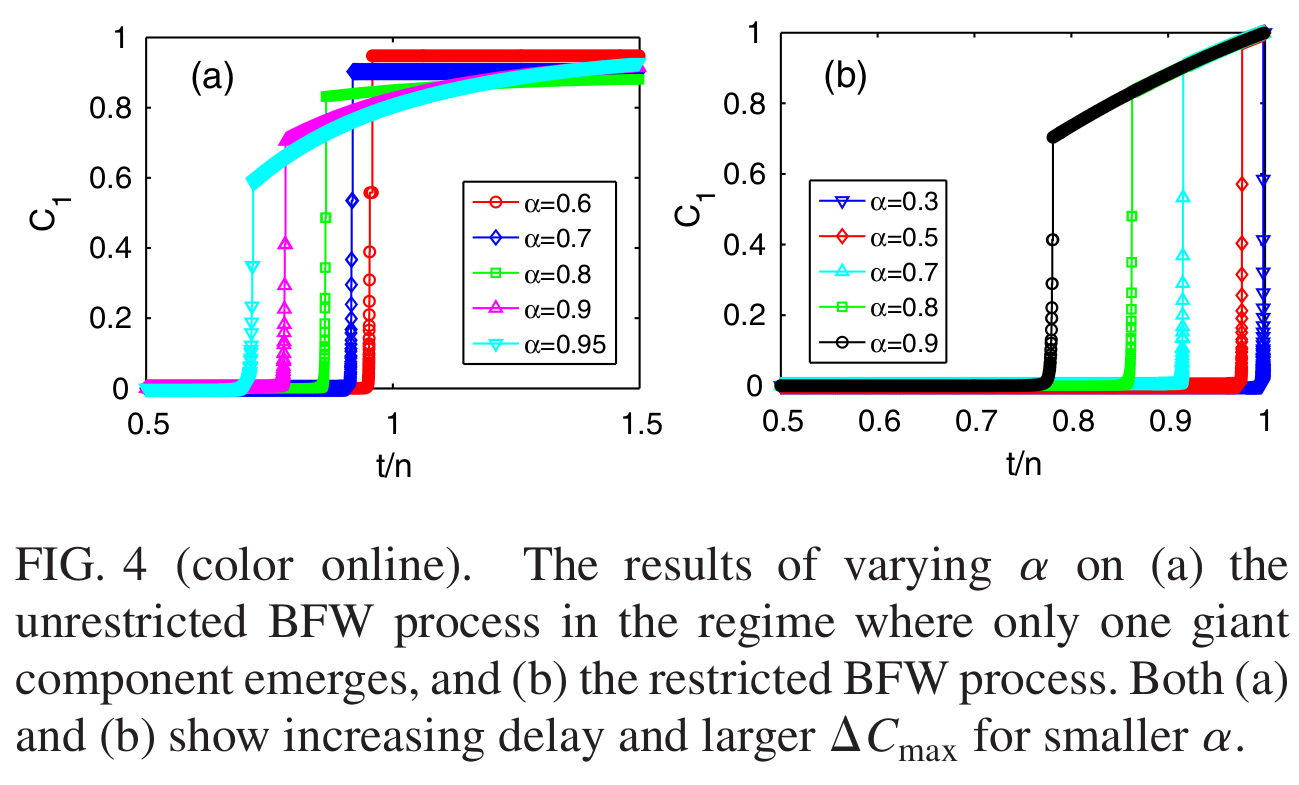
\includegraphics[width=350pt]{images/bfw_alpha_comparison.png}
	\caption{Phase transition dependence on $\alpha$. Source: \cite{Chen_1}.}
	\label{fig:bfw_alpha_comparison}
\end{figure}

Their analysis shows that it is possible to have multiple stable giant components emerge at the same critical point.
Furthermore they finish their paper by stating that the BFW model is strongly discontinuous.



\subsubsection{Continuity With Unusual Finite-Size Scaling Behavior}
In 2011 Grassberger et al. published "Explosive Percolation is Continuous, but with Unusual Finite Size Behavior" \cite{Grassberger_1} in which they studied the phase transitions of four different Achlioptas processes.
They specifically looked at the distribution $P_{r, N}(m)$ of the order parameter $m = |C| / N$, and at the critical point it scales as:

\begin{equation}
	P_{r=r_c, N}(m) \sim N^\eta f(m N^\eta)
\end{equation}
In the Ising model (continuous transition) the function $f(z)$ has two peaks and as $N \rightarrow \infty$ the peaks move closer together to form a single peak, whereas in a first order transition $f(z)$ is double peaked and the peaks move further apart as $N \rightarrow \infty$.
The finite size scaling of $\langle m \rangle$ is given by:

\begin{equation}
	\langle m \rangle \sim (r - r_c)^\beta g((r - r_c) N^\Theta)
\end{equation}
$g(z)$ is analytic for all $z \in \mathbb{R}$.

\begin{figure}[H]
	\centering
	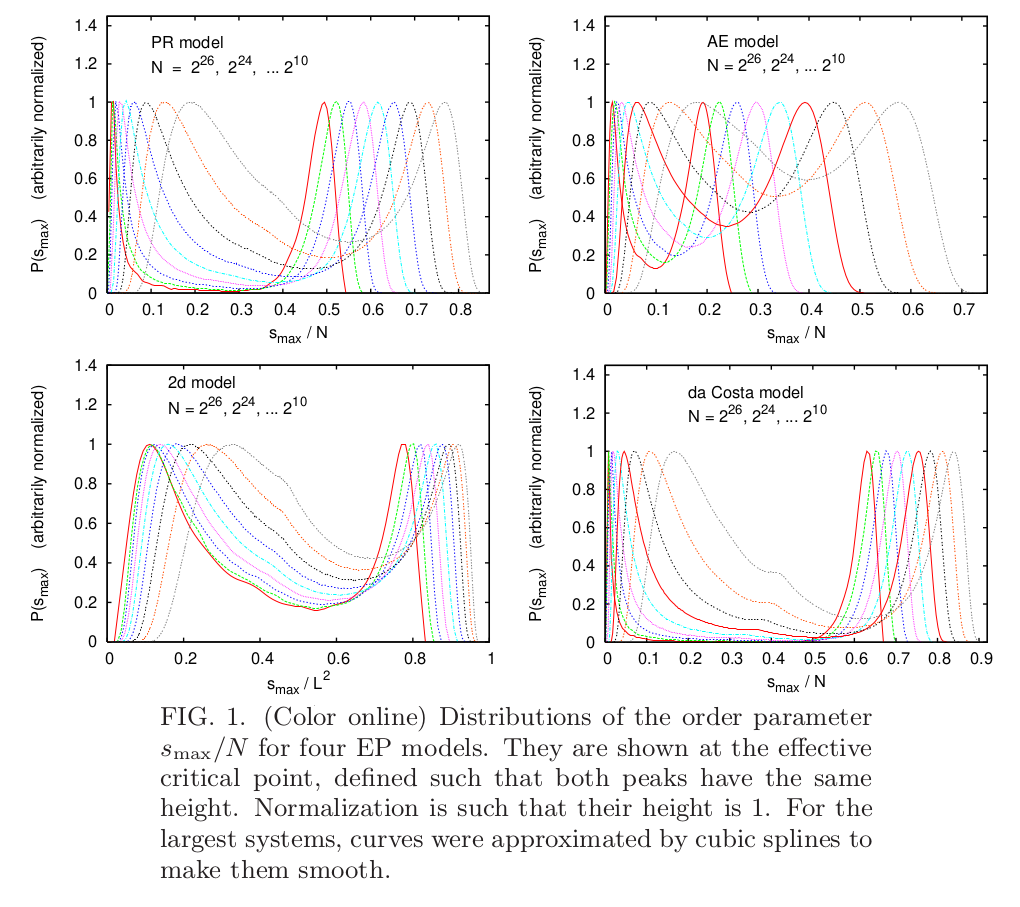
\includegraphics[width=350pt]{images/grassberger_scaling.png}
	\caption{Scaling of $P_{r=r_c, N}(m)$. Source: \cite{Grassberger_1}.}
	\label{fig:grassberger_scaling}
\end{figure}

Their results shown in Fig. \ref{fig:grassberger_scaling} showed that $P_{r=r_c, N}(m)$ was indeed double peaked, however, they say that this does not prove it is continuous, rather it reflects how abruptly the system transitions.
They then go on to show (through the use of FSS of $\langle m \rangle$) that the transitions of the studied four models are indeed continuous, yet are each in a different universality class and all exhibit unusual finite size scaling behavior.



\subsubsection{Large Scale Simulations Show It's Continuous}
The 2011 paper "Continuity of the Explosive Percolation Transition" \cite{Lee_1} by Hyun Keun Lee, Beom Jun Kim, and Hyunggyu Park analyzed the finite-size scaling of the product rule in depth, using data from simulations of system sizes up to $2^{37} \approx 1.4 \cdot 10^{11}$.
They use a fairly straightforward method for determining the continuity of the transition:

\begin{enumerate}
	\item Set $t_0(N) < t_c$ and $t_1(N) > t_c$ with the expectation that as $N \rightarrow \infty$, $t_0 \rightarrow t_c$ and $t_1 \rightarrow t_c$.
	\item Find an upper bound for the change in the largest cluster size $\Delta |C|$.
	\item Show that $\Delta |C|$ scales sublinearly with $N$.
\end{enumerate}

Near the end they arrive at:

\begin{equation}
	\Delta m = \frac{\Delta |C|}{N} \lesssim N^{-0.022}
\end{equation}
Which means that as $N \rightarrow \infty$, $\Delta m \rightarrow 0$ and they conclude that the transition is indeed continuous.



\subsubsection{Proof of Continuity Emerges}
Oliver Riordan and Lutz Warnke published "Achlioptas Process Phase Transitions Are
Continuous" \cite{Riordan_1} in 2012, wherein they lay out several theorems and proofs to show that all Achlioptas processes result in a continuous phase transition.
Due to the long and detailed nature of the proofs the reader is referred to their work for further information.



\subsubsection{"Solution of the explosive percolation quest"}
In 2014 and 2015 Rui da Costa, Sergey Dorogovtsev, Alexander Goltsev, and Jose Fernando Mendes published three more papers \cite{da_Costa_5, da_Costa_2, da_Costa_3} where they performed a significant amount of research on the explosive percolation transition of the $q$-edge model laid out in their previous paper (see above \textbf{No, It's Actually Continuous!}).

In "Critical exponents of the explosive percolation transition" \cite{da_Costa_5} they study extensively the critical exponents and how they scale as $q$ changes, wherein they observe that as $q$ increases $\beta$ quickly declines, with $\beta(q = 4) \approx \beta(q = 2) / 20$.
They talk about how models that only use local information, i.e. they do not require knowledge of all of the clusters within the graph but only those corresponding to the candidate edges, lead to a continuous transition, but models that take global information into account might lead to discontinuities.

In "Solution of the explosive percolation quest: Scaling functions and critical exponents" \cite{da_Costa_2}
and "Solution of the explosive percolation quest. II. Infinite-order transition produced by the initial distributions of clusters" \cite{da_Costa_3} they develop a thorough theory of finite-size scaling that explains the continuity of the transition.
Their theory is quite extensive and worth the read.



\subsubsection{A Look At the Developments}
After seeing a number of papers stating that the transition is actually continuous, it looked like the debate had been settled.
$q$-edge Achlioptas processes are always continuous if they only take local information into account, but there exist some processes that take global information into account that lead to a discontinuous transition.
A lot of different rules for selecting, evaluating, and adding edges were created and in the 2015 paper "Explosive Percolation: Novel critical and supercritical phenomena" \cite{D_Souza_2} by Raissa M. D’Souza and Jan Nagler summarized a lot of the developments and findings in the field up to that point.
They discussed similarities and differences between some of the well known explosive percolation models and tied it all together nicely with some real world applications and future directions for the field.
Overall it is an excellent paper to read to get acquainted with how the field developed from 2009 to 2015.


\chapter{A New Model}
\label{ch:sea}
\section{Stochastic Edge Acceptance}
After reading a lot about other models for evolving graphs I decided to come up with a new model for adding edges with an extra element of randomness.
The model is called Stochastic Edge Acceptance or SEA for short.
In most models the edges selected for evaluation are random but which of those edges is added to the graph is deterministic like in the product rule where the one with the smallest product is always accepted.

The underlying idea is to have a process which favors the minimization of the largest cluster through considering multiple edges at each step in the evolution algorithm, making it an Achlioptas process.
This is a local rule, i.e. it only considers local information such as the size of the clusters to which the nodes corresponding to the considered edges belong.
I wanted to create a simple probability using only the sizes of the clusters corresponding to the considered edges.
Using just the cluster size information it is easy to create a set of probabilities that decrease as the cluster size increases.
The way it is designed actually allows us to generalize this algorithm to evaluate $q$ edges at once with corresponding probabilities $p_i$, $i \in \{1, 2, ..., q\}$:

\begin{equation}
	p_i = \frac{\frac{1}{|C_i|}}{\sum_j \frac{1}{|C_j|}}
\end{equation}

A form of the algorithm for $q = 2$ can be written in pseudocode as follows:
\begin{itemize}
	\item Let $T$ be the total number of edges to add to the graph.
	\item Let $A_t = \{e_1, e_2, ..., e_t\}$ be the set of accepted edges at step $t$.
	\item Let $e_t^1$ and $e_t^2$ be the two nodes which edge $e_t$ would connect.
	\item Let $C(e_t^i)$ be the cluster which $e_t^i$ belongs to.
	\item Let $C(e_t)$ be the cluster which would be formed by activating $e_t$.
	\item Let $R \in [0, 1)$ be a randomly generated number.
\end{itemize}

\begin{algorithm}[H]
	\caption{Stochastic Edge Acceptance}\label{Stochastic-Edge-Acceptance}
	\begin{algorithmic}[1]
		\Procedure{SEA}{$T$}
		\State $A \gets \emptyset$
		\State $t \gets 1$

		\While{$t \le T$}
			\If{$C(e_t^1) = C(e_t^2)$}
				\State $A \gets A \cup \{e_t\}$
				\State $t \gets t+1$
			\ElsIf{$C(e_t'^1) = C(e_t'^2)$}
				\State $A \gets A \cup \{e_t'\}$
				\State $t \gets t+1$
			\ElsIf{$p$ > R}
				\State $A \gets A \cup \{e_t\}$
				\State $t \gets t+1$
			\Else
				\State $A \gets A \cup \{e_t'\}$
				\State $t \gets t+1$
			\EndIf
		\EndWhile
	\EndProcedure
	\end{algorithmic}
\end{algorithm}

The $q$-edge algorithm is similar except it would use a cumulative probability $P_i = \sum\limits_{j=1}^{i} p_i$ (much like in the $q$-state Potts model) and loop over $i \in \{1, 2, ..., q\}$ until $P_i > R$, and then once that is satisfied accept the edge and move to the next step.



%---------------------------------------------------------------------------------------
% Simulation and Analysis
%---------------------------------------------------------------------------------------
\subsection{Simulation and Analysis}
All data in this section was generated using GraphEvolve.jl (see appendix for more information).
Random networks of sizes $2^k$, $k \in \{15, 16, ..., 24\}$ were studied, and for each system size 1000 simulations were run with different random number generator seed values.
It would be ideal to run simulations for larger system sizes to get a more representative sample, and is something which can be investigated further in the future.
All code and the associated generated data used for this is publicly available on the corresponding GitHub page \url{https://github.com/cameronperot/explosive-percolation}.

Fig. \ref{fig:ER_BF_PR_SEA_transition} illustrates the order parameter of the SEA model in comparison with the ER, BF, and PR models.
The SEA model experiences a transition later than the ER and BF models, but before the PR model.
The order parameter shows a sharp increase at the point of phase transition with an almost vertical slope similar to that of the PR.

\begin{figure}[H]
	\centering
	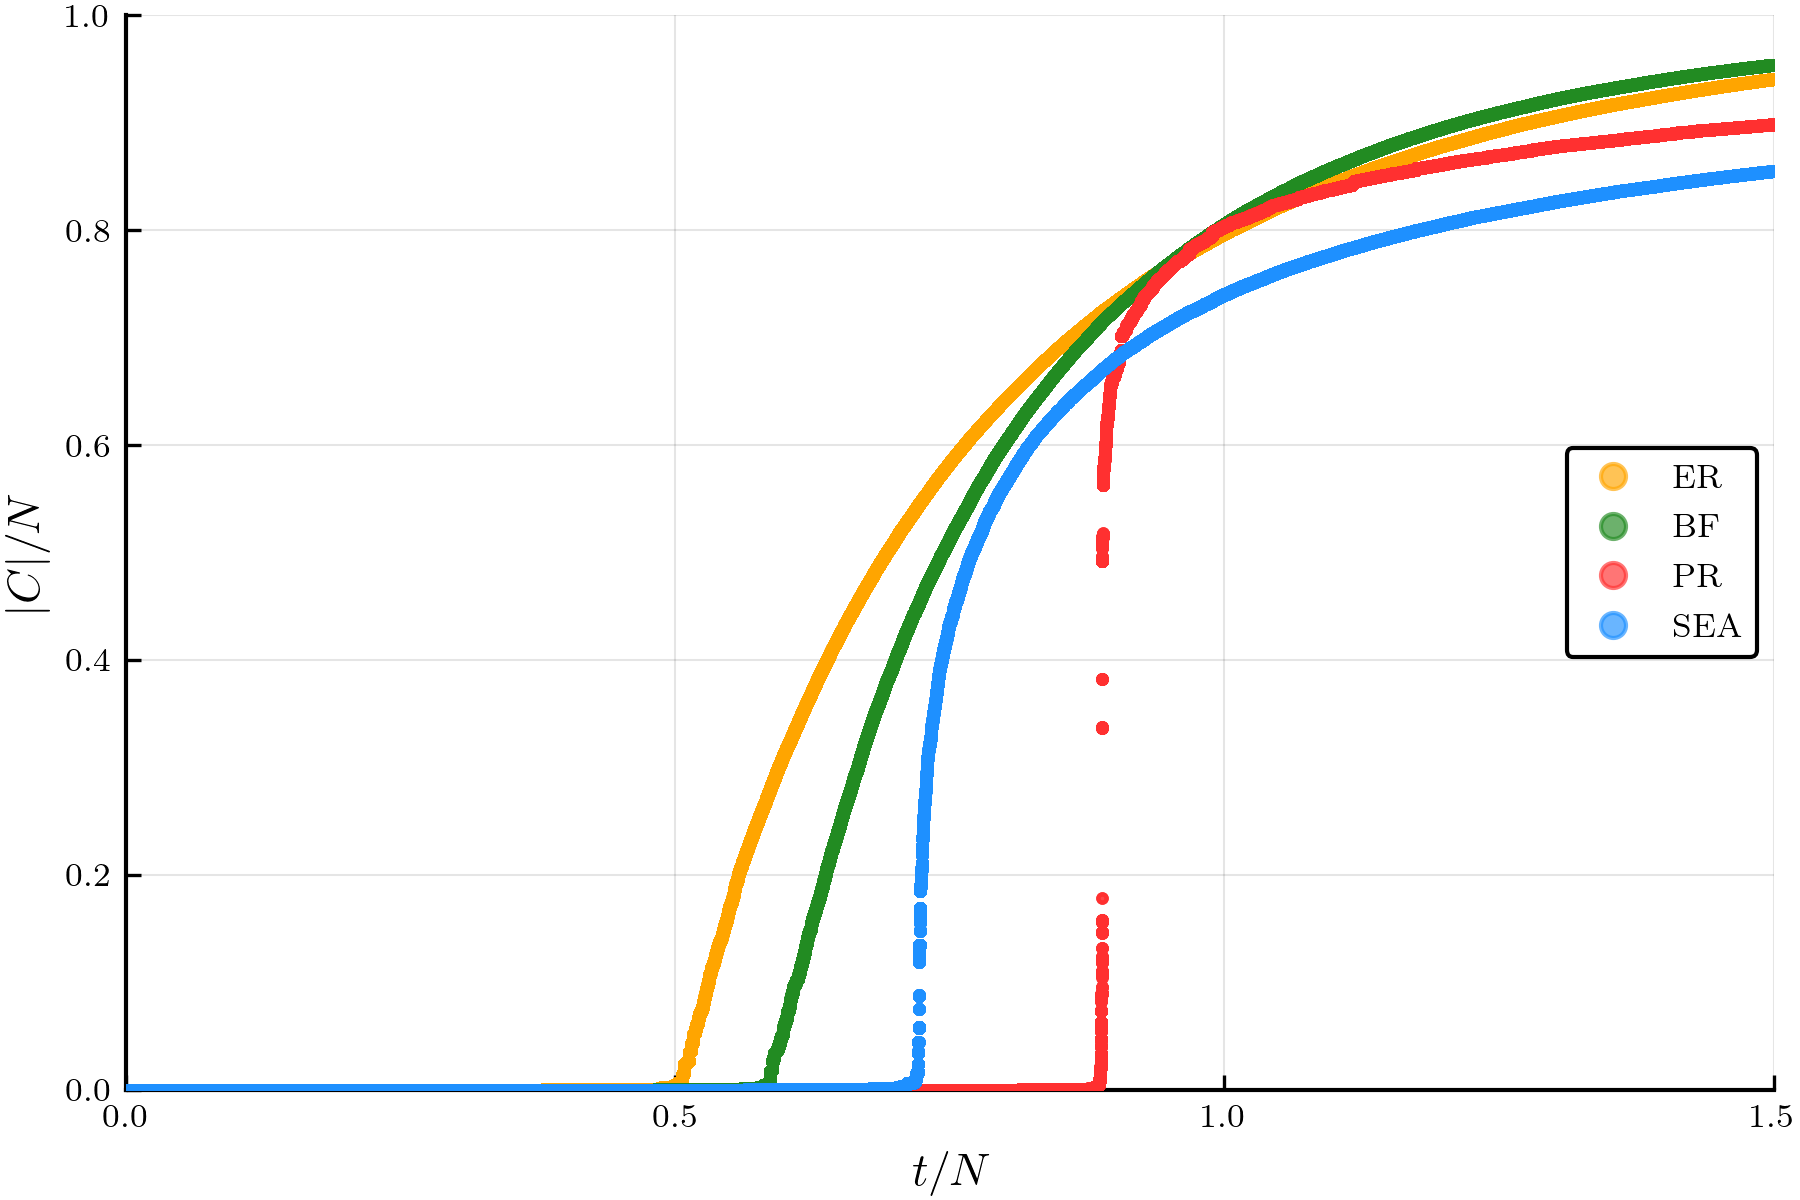
\includegraphics[width=350pt, clip]{images/Network_ER_BF_PR_SEA_1e6_order_param.png}
	\caption{Comparison of the stochastic edge acceptance order parameter to that of well-known models ER, BF, and PR. $N = 10^6$.}
	\label{fig:ER_BF_PR_SEA_transition}
\end{figure}

\begin{figure}[H]
	\centering
	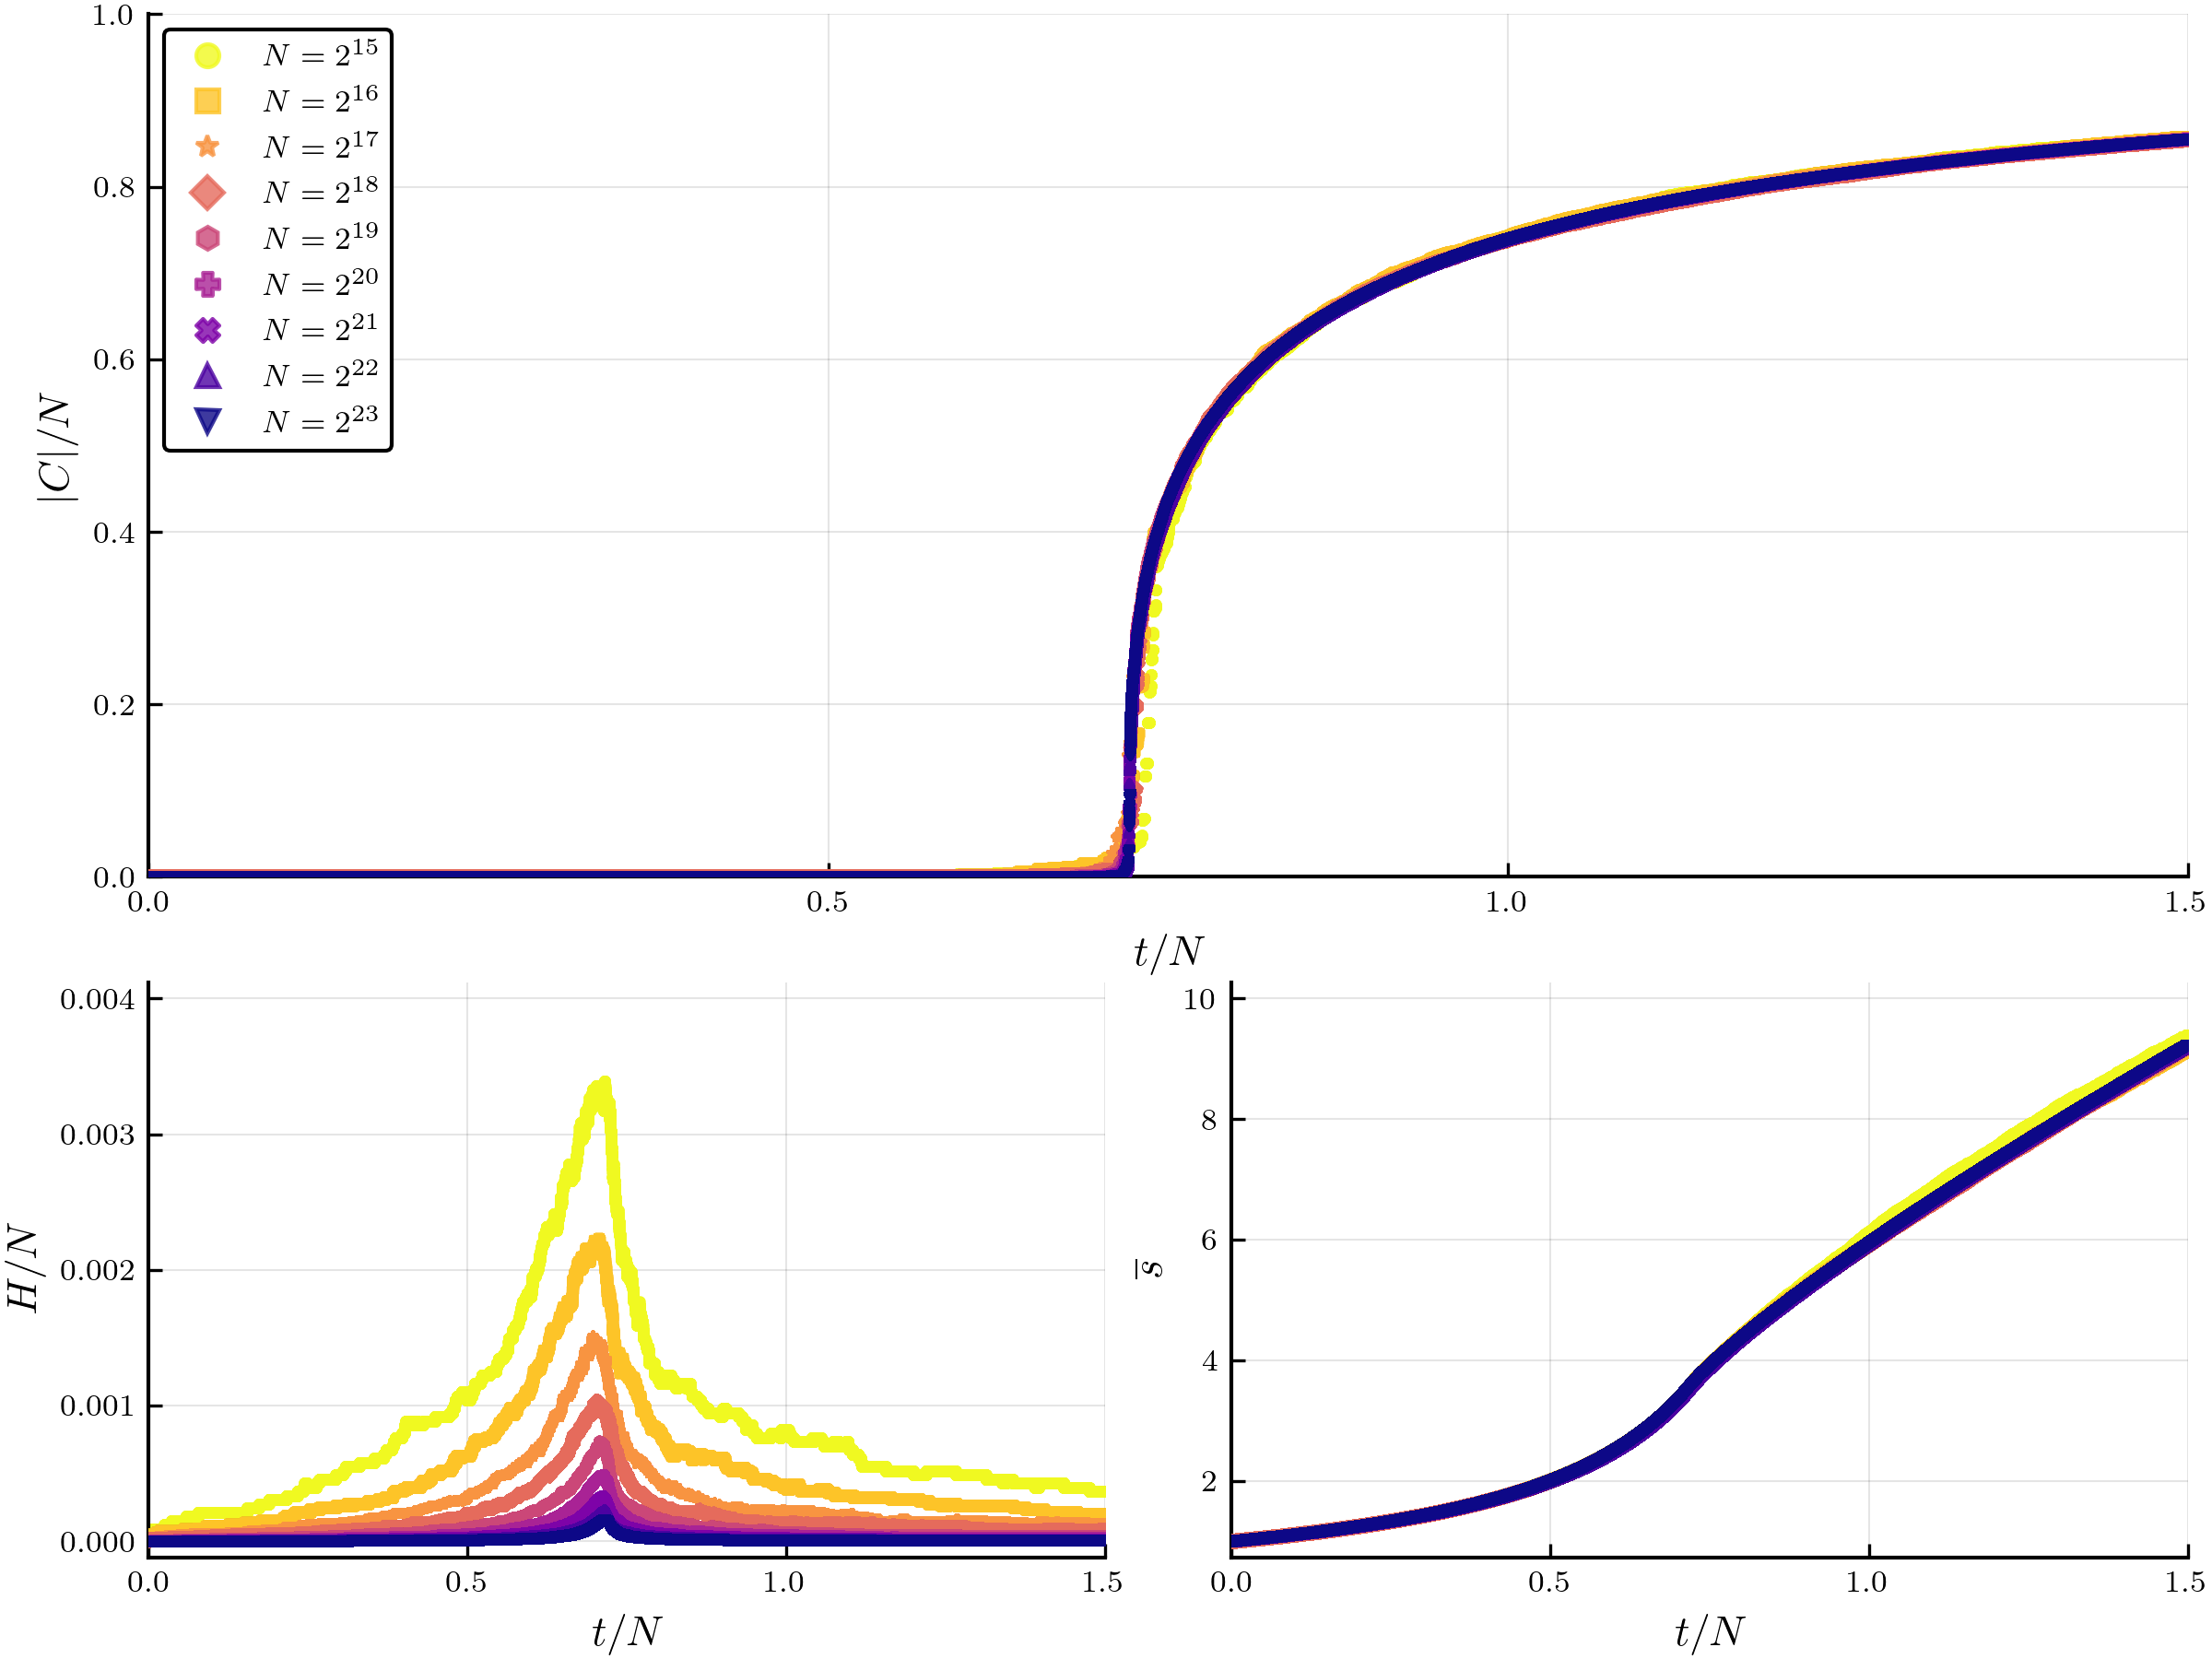
\includegraphics[width=350pt, clip]{images/k_scaling_triple.png}
	\caption{Observables dependence on system size. $H$ is the cluster heterogeneity and $\overline{s}$ is the average cluster size. As the system size increases the the peak of the heterogeneity per node $H/N$ decreases and moves towards the right. The average cluster size lines up for all system sizes.}
	\label{fig:k_scaling_triple}
\end{figure}

Now that we've seen it exhibits interesting behavior at the point of phase transition we would like to learn more such as where does it transition, and most importantly, is it continuous?
In order to answer these questions we will use the framework laid out in \cite{Lee_1}.
First we need to find two points, one before the transition ($t_0$) and one after the transition ($t_1$).
We set $t_0$ as the point at which the cluster heterogeneity peaks, i.e. when the number of unique cluster sizes is at its highest.
We set $t_1$ as the point at which the order parameter experiences its largest increase.
Let $r_i = t_i / N$ represent the relative number of edges in the system at step $t_i$ (because at step $t_i$ there are $t_i$ edges present in the graph), and $m_i = m(r_i)$ be the order parameter at step $t_i$.
We will define two quantities which we would like to study the behavior of:

\begin{equation}
\begin{split}
	\Delta r &= r_1 - r_0 \\
	\Delta m &= m_1 - m_0
\end{split}
\end{equation}

Fig. \ref{fig:r_scaling} shows the scaling behavior of $r_0$ and $r_1$ as a function of the system size $N$.
As the system size increases the two curves appear to be to be converging to the exact point of phase transition.
The obtained data tells us that the system transitions phases around $r \approx 0.718(4)$.

\begin{figure}[H]
	\centering
	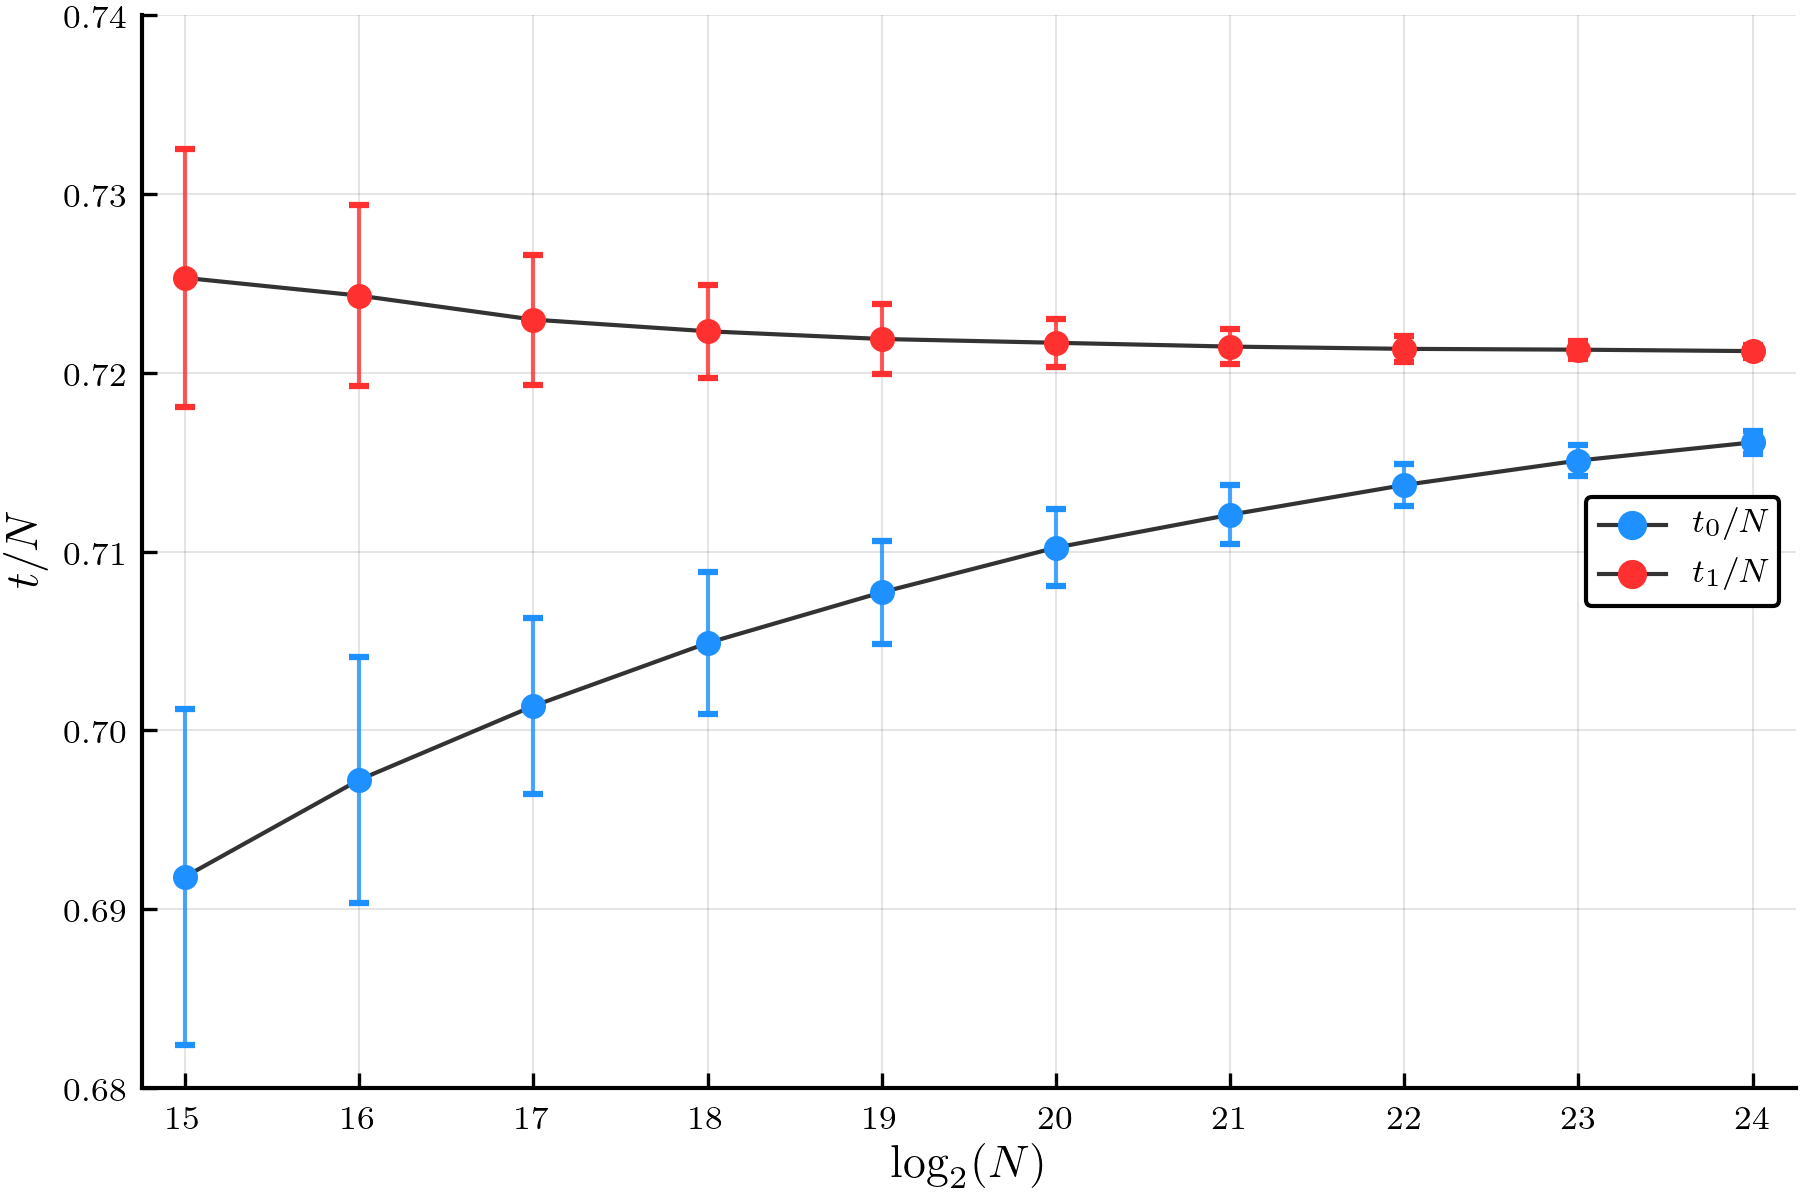
\includegraphics[width=350pt, clip]{images/r_scaling.png}
	\caption{The curves for $r_0$ and $r_1$ appear to be converging to the point of phase transition.}
	\label{fig:r_scaling}
\end{figure}

When looking at the scaling behavior of certain quantities it often helps to view them on $\log-\log$ plots to identify any power law scaling behavior.
Fig. \ref{fig:delta_r_scaling} shows $\Delta r$ as a function of the system size, and as we can see it exhibits power law scaling behavior of the form:

\begin{equation}
	\Delta r \sim N^{-\delta}
\end{equation}
with $\delta \approx 0.302(2)$.

\begin{figure}[H]
	\centering
	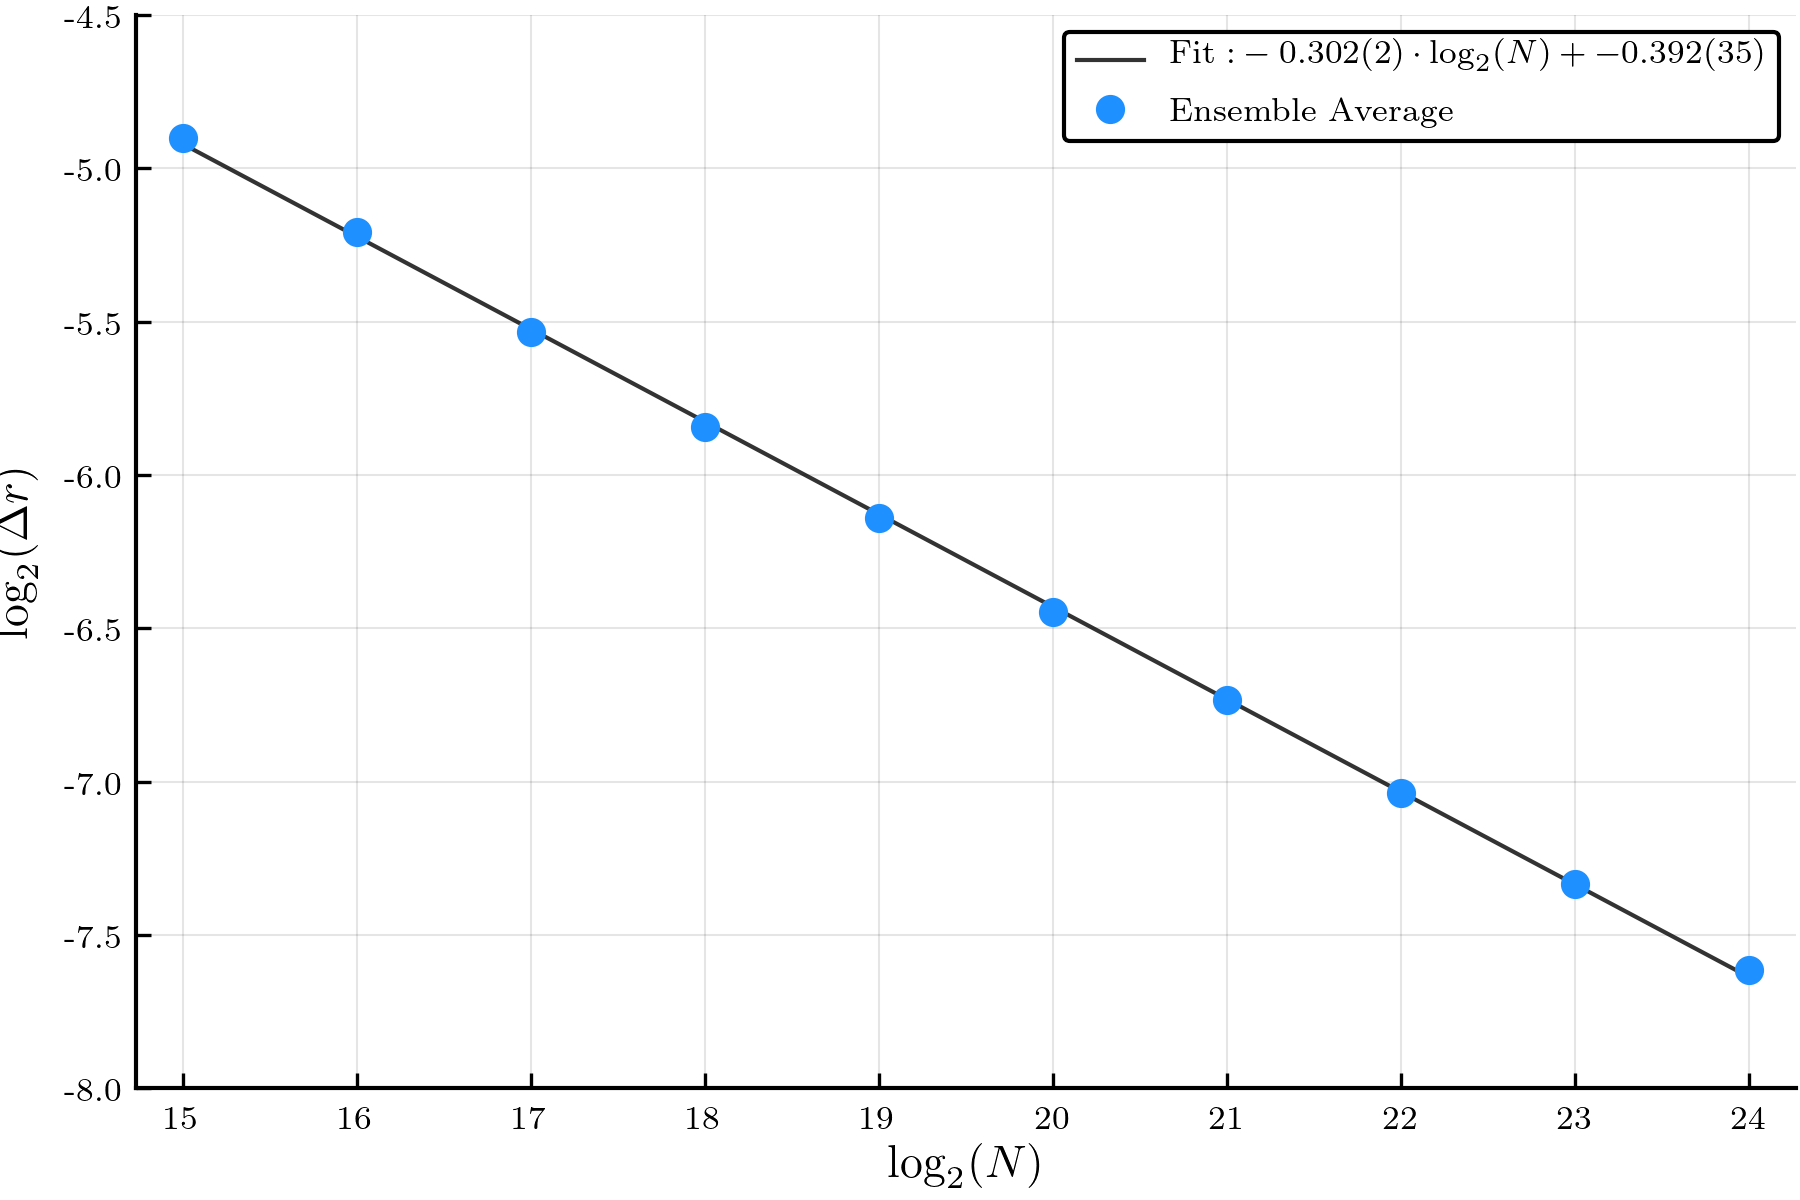
\includegraphics[width=350pt, clip]{images/delta_r_scaling.png}
	\caption{$\Delta r$ exhibits power law scaling in $N$.}
	\label{fig:delta_r_scaling}
\end{figure}

There is a lot of information contained in the cluster size distributions at $t_0$ and $t_1$.
We first start by analyzing the distribution at $t_0$, shown in Fig. \ref{fig:n_s_t_0}.

\begin{figure}[H]
	\centering
	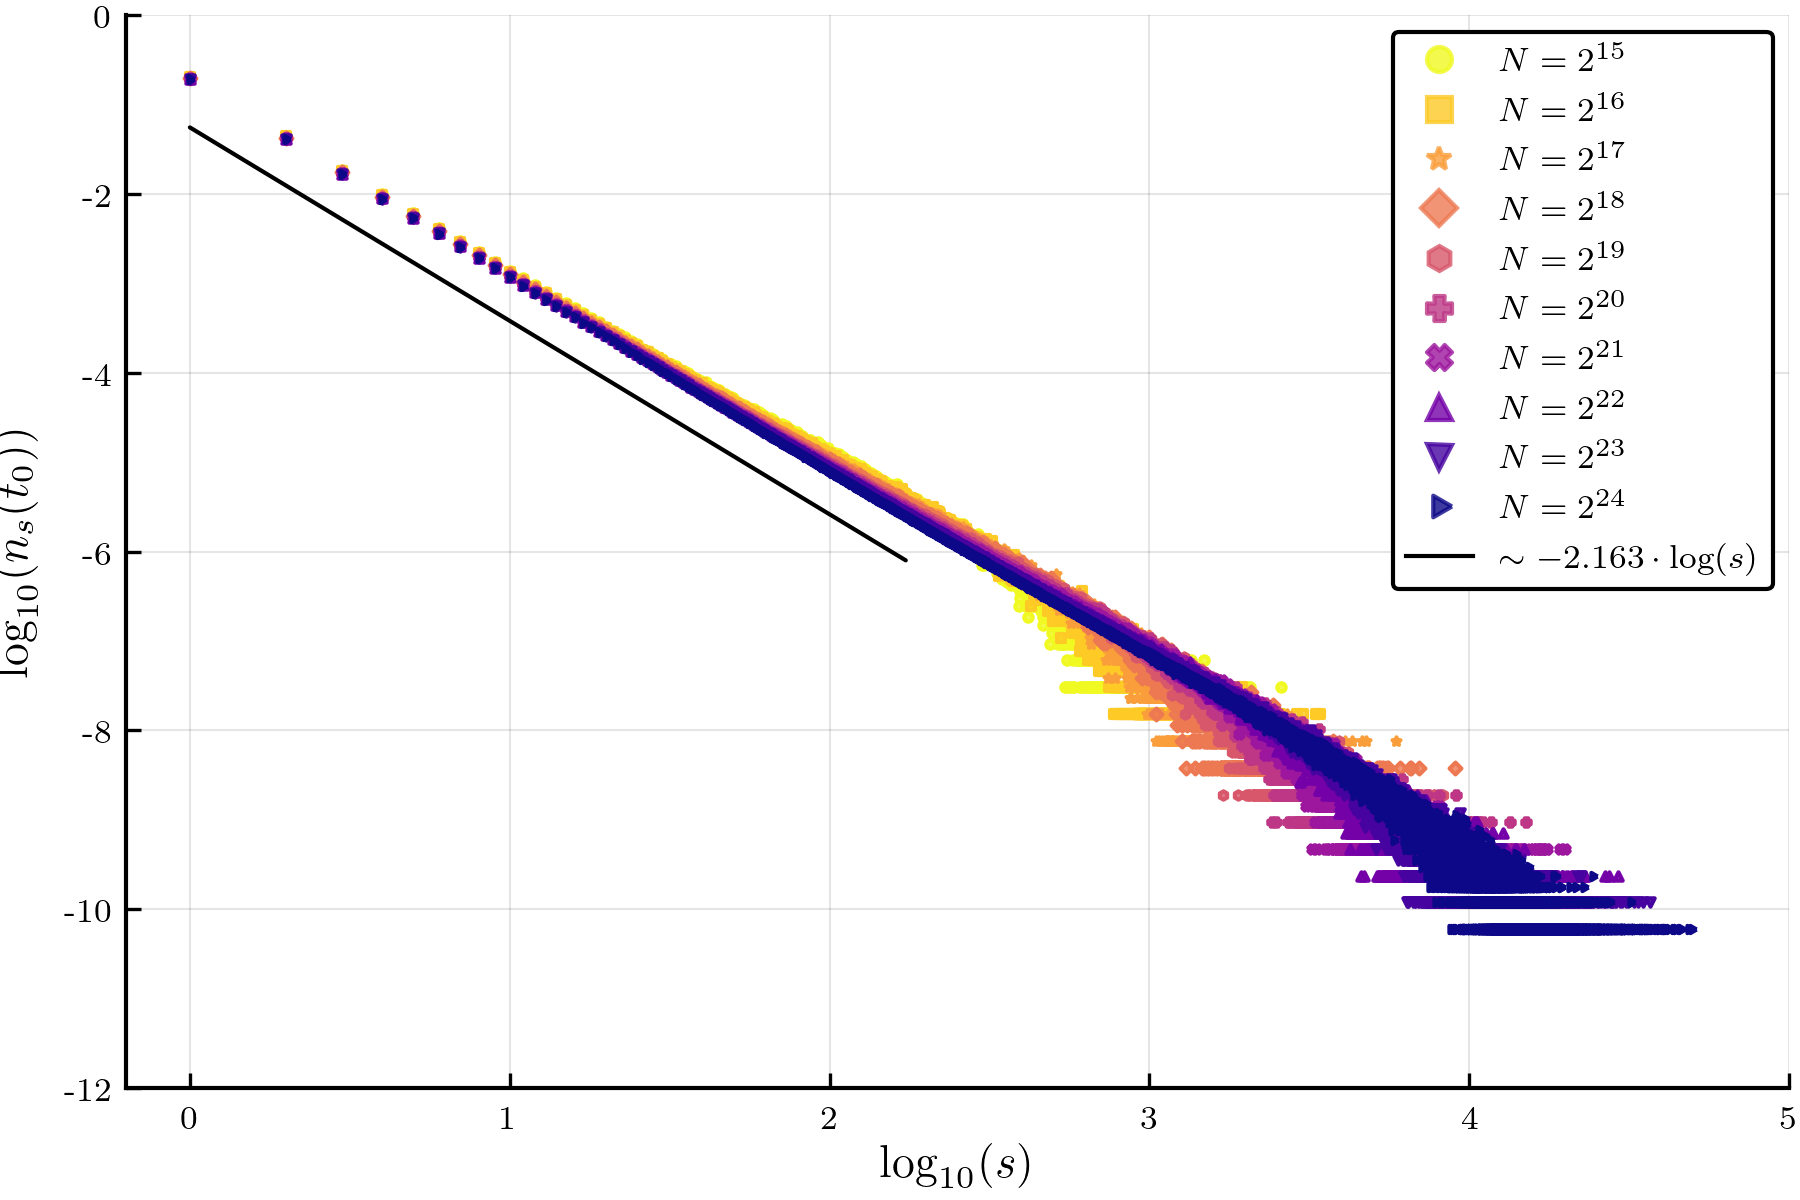
\includegraphics[width=350pt, clip]{images/n_s_t_0.png}
	\caption{Scaling behavior of the cluster size distribution at $t_0$.}
	\label{fig:n_s_t_0}
\end{figure}
When plotted on a $\log_{10}-\log_{10}$ basis we see a linear relationship up to a certain cutoff cluster size $s_f$ where $n_s(t_0)$ then drops off exponentially.
Large statistical errors are visible for higher values of $s$, but nevertheless the overall message of the plot is clear.
This linear behavior tells us this is a power law in $N$ and using the ansatz:

\begin{equation}
	n_s(t_0) \sim s^{-\tau}
\end{equation}
and performing a linear fit gives us the value of the exponent $\tau_0 \approx 2.163$.

Looking at the data for the cluster size distribution at $t_1$ (Fig. \ref{fig:n_s_t_1}) we see a similar power law scaling relation, except with a slightly different exponent $\tau_1 \approx 2.218$.
I believe the discrepancy in the exponents here is due to the size of the simulations, and that if simulated with larger system sizes (such as up to $2^{37}$ seen in \cite{Lee_1}) that the values would converge towards the true value of $\tau$.
In Fig. \ref{fig:n_s_t_1} we see $\log_{10}(n_s(t_1))$ versus $\log_{10}(s/N)$ rather than just $\log(s)$, where we again observe this linear scaling up to a point ($s_f$) where it then dips and breaks the linear trend (once again large statistical errors for larger values of $s/N$).

\begin{figure}[H]
	\centering
	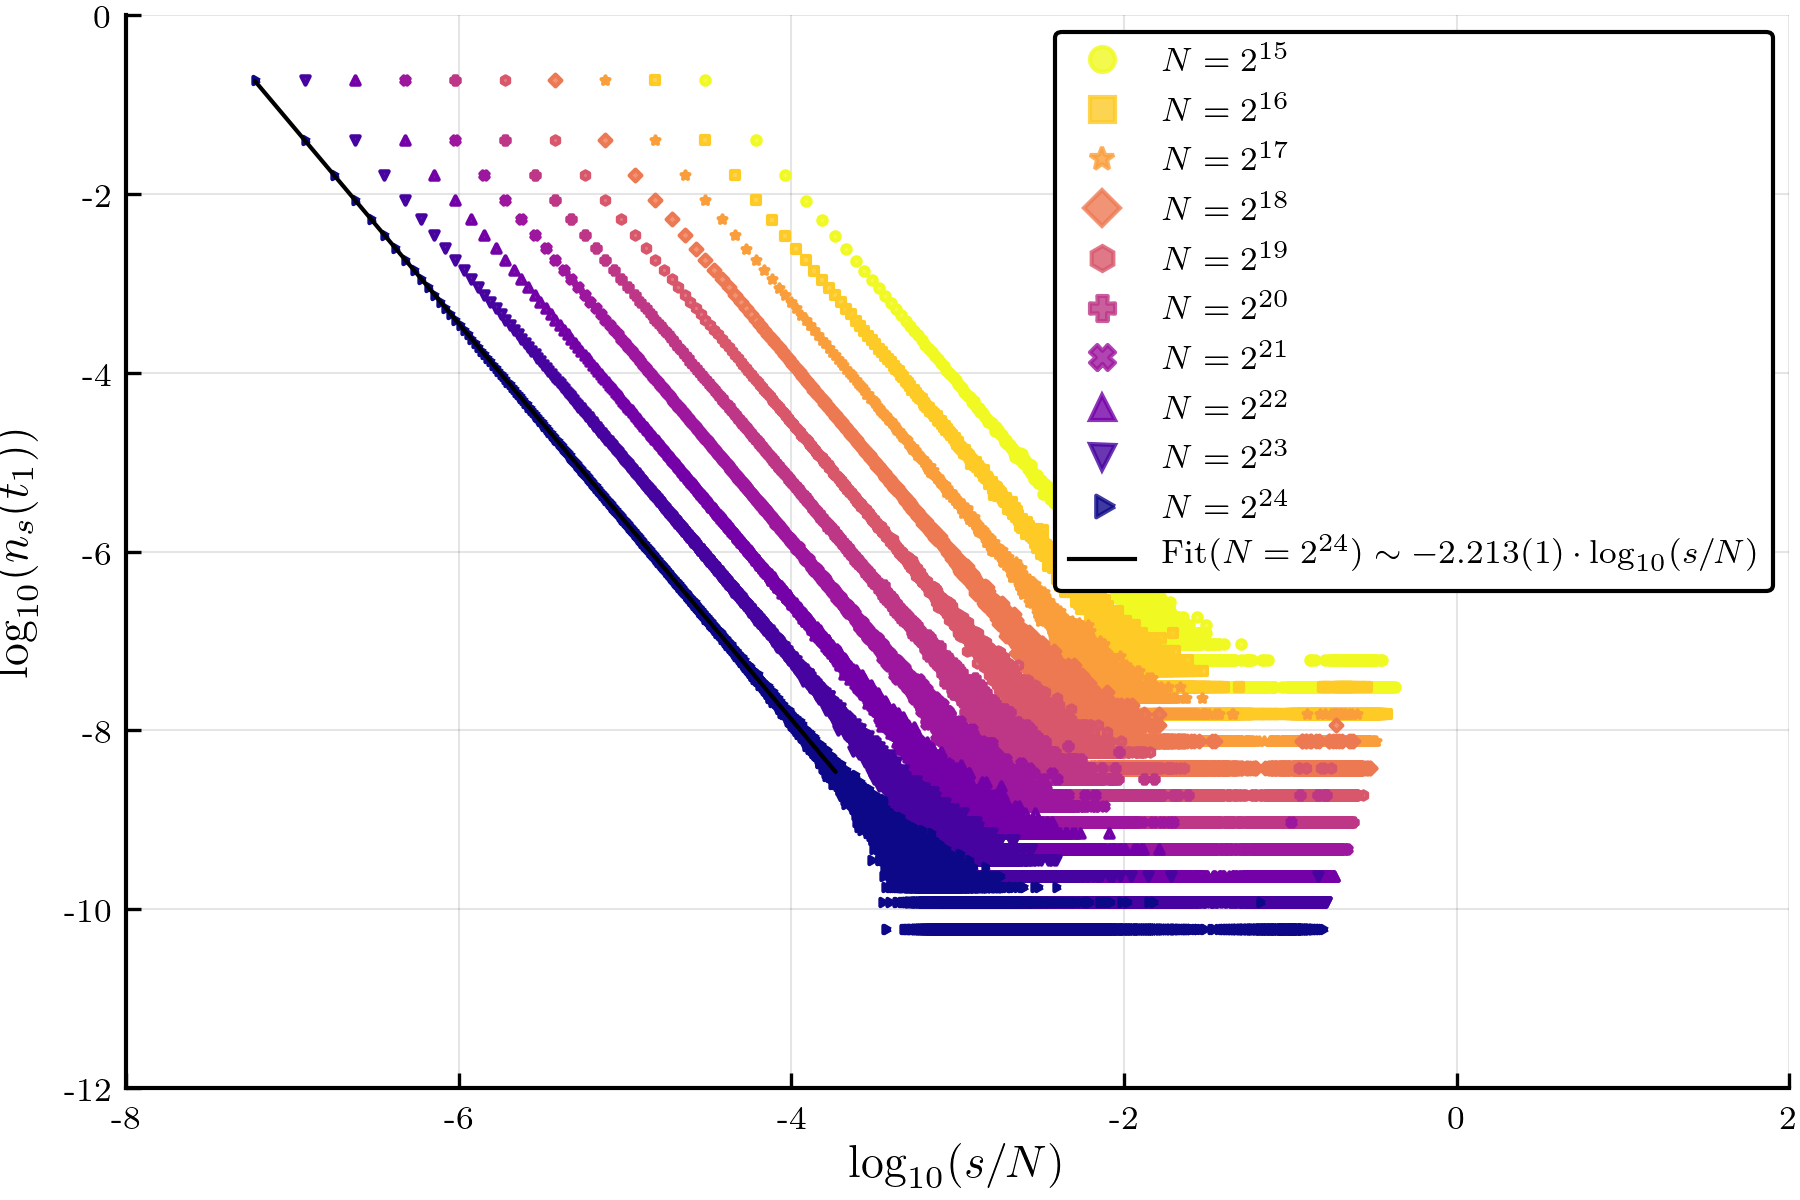
\includegraphics[width=350pt, clip]{images/n_s_t_1.png}
	\caption{Scaling behavior of the cluster size distribution at $t_1$.}
	\label{fig:n_s_t_1}
\end{figure}

In \cite{Lee_1} they determine $s_f$ by taking the ansatz $\sum_{s \ge s_f} \sim 1 / N_{C, 0}$ where $N_{C, 0}$ is the total number of clusters at $t_0$.
Then through the use of several relations such as the the number of clusters scaling linearly with the system size they arrive at:

\begin{equation}
	s_f(N) \sim N^{1 / \tau}
\end{equation}

This can be verified by assuming a single characteristic cluster size and taking the finite-size scaling form of $n_s$ \cite{Lee_1}:

\begin{equation}
	n_s(t_0) = s^{-\tau} f(s / s_f) = s^{-\tau} f(s N^{-1 / \tau})
\end{equation}

Applying this same ideology to the stochastic edge acceptance method works quite well as seen in Fig. \ref{fig:fss_collapse_triple}.
This verifies that indeed $\tau_1 \approx 2.218$ is a good estimation of $\tau$ as the plot shows that the data for all of the system sizes lines up well and exhibits this hump behavior also seen in \cite{Lee_1}.
The data analysis up to this point leads me to believe that the discrepancies in the fitted values of $\tau$ could be due to $t_1$ being closer to the critical point than $t_0$, and as $N$ increases we see $t_0$ move closer to $t_1$ (Fig. \ref{fig:r_scaling}), thus if we ran simulations with larger values of $N$ then we should be able to obtain a more accurate reading of $\tau$.

\begin{figure}[H]
	\centering
	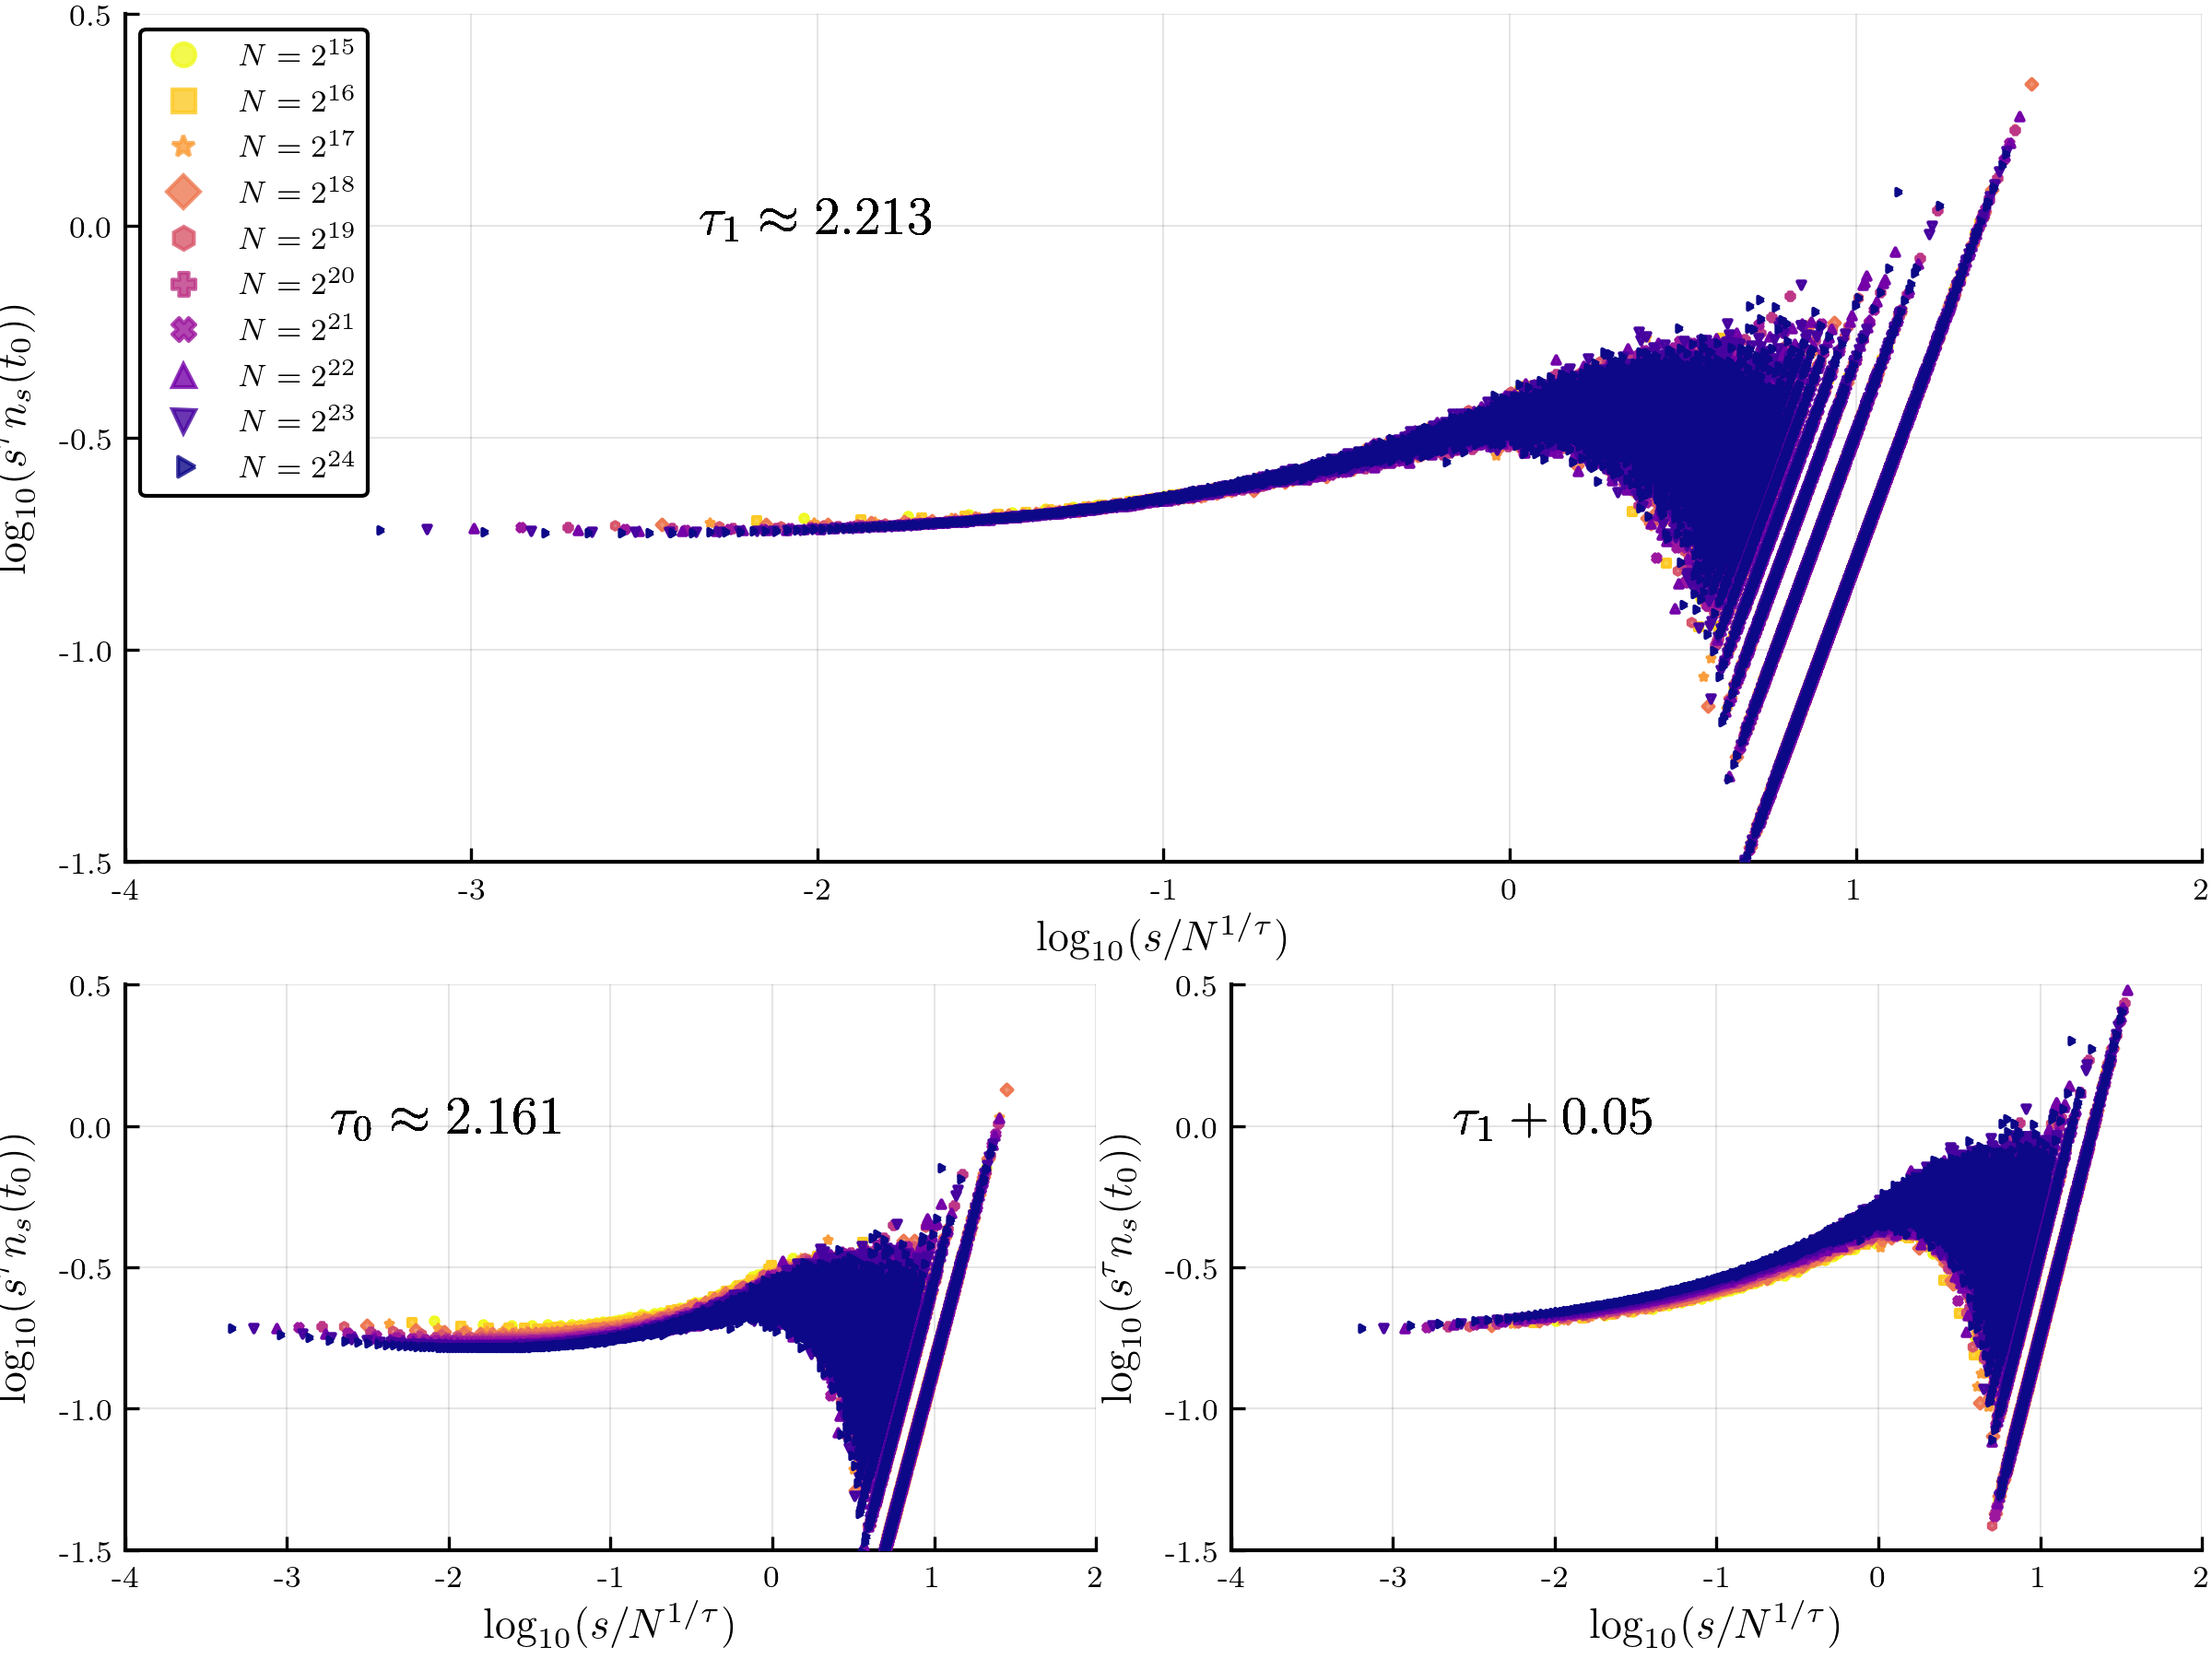
\includegraphics[width=350pt, clip]{images/fss_collapse_triple.png}
	\caption{$n_s(t_0)$ finite-size scaling shows a collapse of the data for the critical exponent value $\tau_1 \approx 2.218$ obtained from fitting the linear portion of the distribution at $t_1$. The lower left plot shows how the collapse looks for the value $\tau_0$ and the lower right plot illustrates a slightly higher value of $\tau$, both of which do not line up as well as when using $\tau_1$.}
	\label{fig:fss_collapse_triple}
\end{figure}

Now that we have extracted some useful information, namely the values of the critical exponents, we want to show is that as the system size tends to infinity that the difference in the order parameter, $\Delta m$, tends to zero, i.e. $\lim_{N \rightarrow \infty} \Delta m = 0$.
In order to show this we want to place an upper bound on $\Delta m$. In \cite{Lee_1} they laid out a clever method for setting an upper bound by starting with the cluster size distribution at $t_0$ and taking an ideal process to add edges in such a way as to maximize the largest cluster size from $t_0$ to $t_1$, thus any other process will produce a $\Delta m$ that is bounded above by the $\Delta m$ produced in the ideal process.
This ideal process would seek to merge all clusters larger than some size $s_\delta$, which is determined by $\Delta t = t_1 - t_0$ and the cluster size distribution at $t_0$, i.e. $\Delta t = N_{C, 0} \sum_{s > s_\delta} n_s(t_0)$, where $N_{C, 0}$ is the total number of clusters at step $t_0$.
What they arrived at is that \cite{Lee_1}:

\begin{equation}
	\Delta m \lesssim s_\delta^{2 - \tau} \sim N^{-\delta (\tau - 2) / (\tau - 1)}
\end{equation}

Plugging in our obtained values of $\delta$ and $\tau$ we find that $\Delta m \lesssim N^{-0.056}$, which implies that the transition of the stochastic edge acceptance model is continuous like other local information based models.
Fig. \ref{fig:delta_m_scaling} shows $\log_2(\Delta m)$ versus $\log_2(N)$ and fitting a line we observe a decay exponent of $0.152(2)$ and verify that this is indeed below the upper bound we arrived at.

\begin{figure}[H]
	\centering
	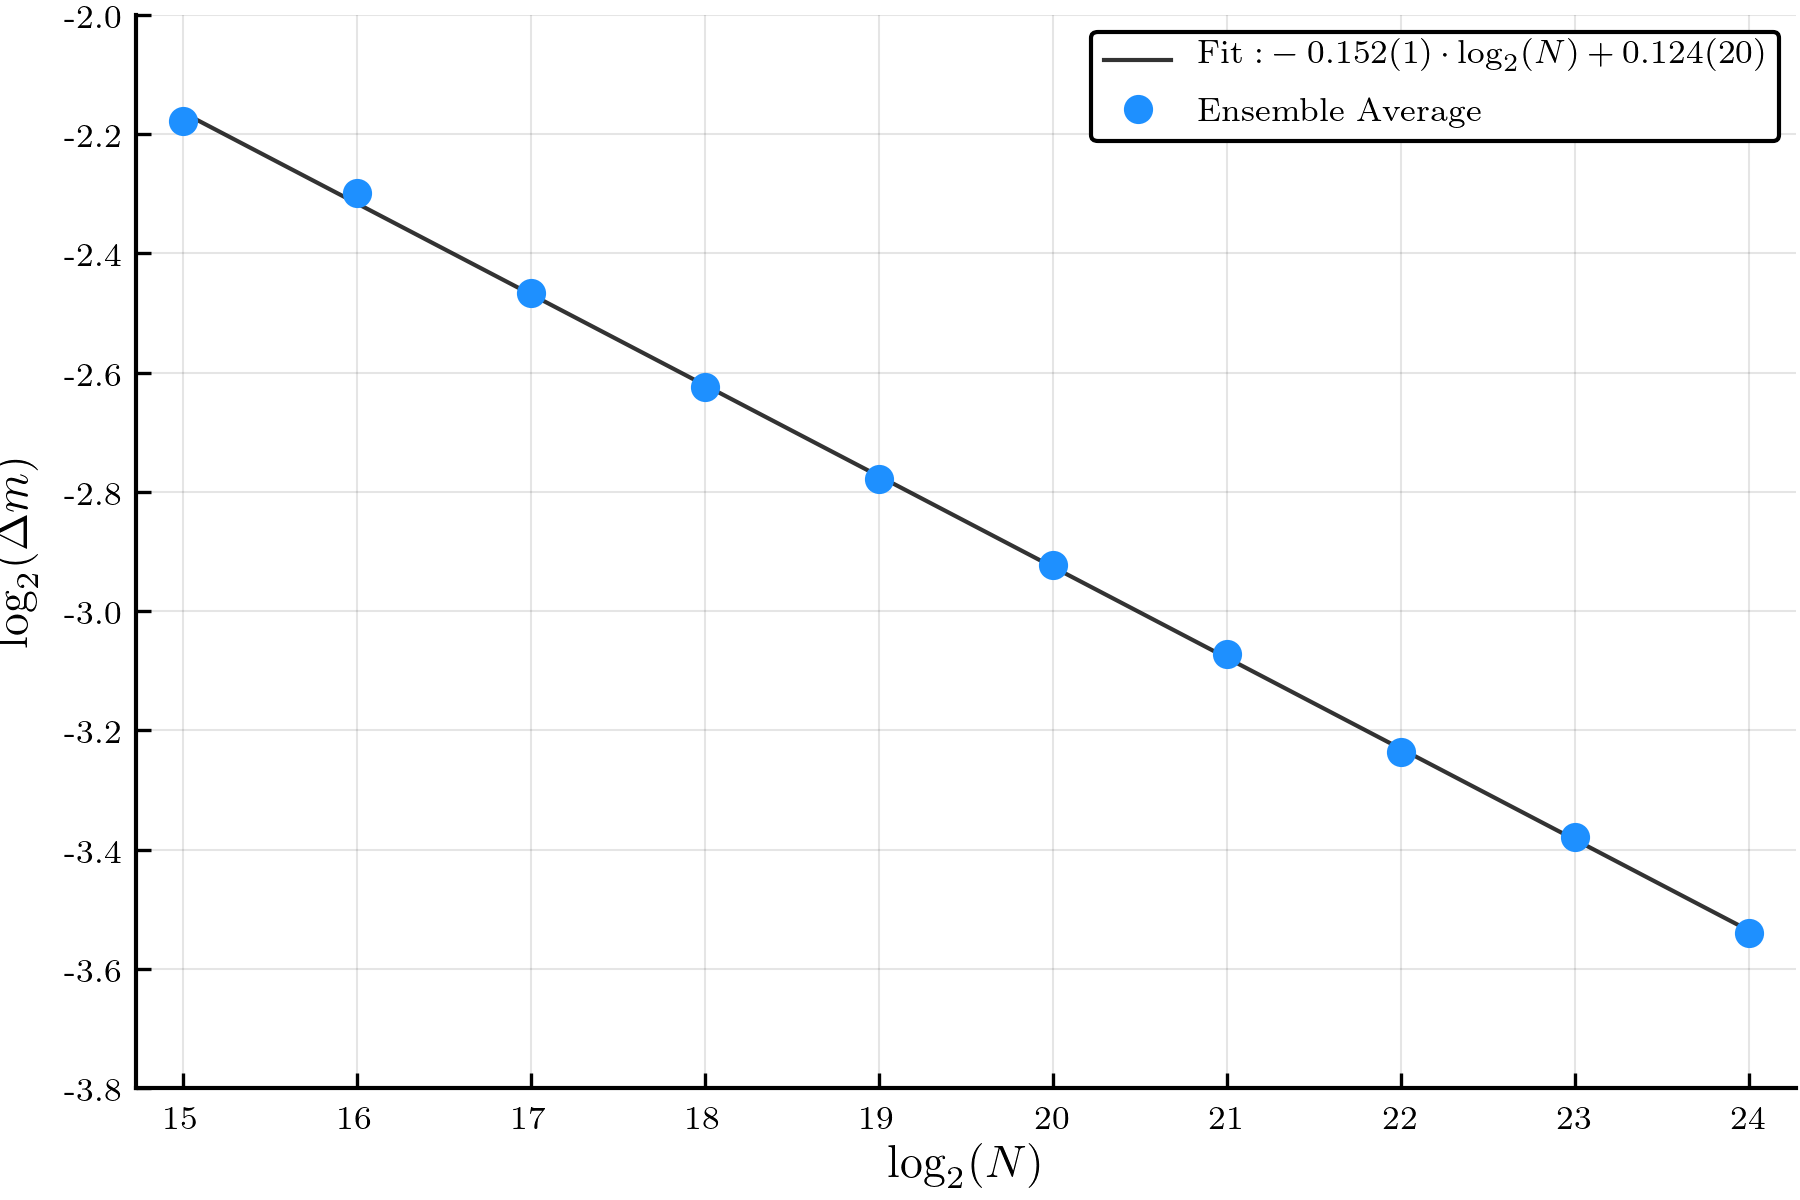
\includegraphics[width=350pt, clip]{images/delta_m_scaling.png}
	\caption{Plotting the change in the order parameter versus the system size on a $\log_2-\log_2$ scale shows that it is well below the upper bound we determined.}
	\label{fig:delta_m_scaling}
\end{figure}



%---------------------------------------------------------------------------------------
% Possible Future Directions
%---------------------------------------------------------------------------------------
\subsection{Possible Future Directions}
There are many different avenues we could go down in the future to further the analysis presented here and in the referenced sources.
The most obvious are studying $q$-edge models for $q \ge 3$ and seeing how the system behaves as $q$ changes, as well as looking at systems other than random networks, such as a lattice.
As a sneak peak, the Figs. below illustrate how the order parameter changes in these scenarios.

Fig. \ref{fig:q_scaling_triple} shows the order parameter for systems of size $N = 10^6$ and $q \in \{2, 3, ..., 7, 8\}$. As we can see, increasing the number of edges evaluated delays the transition even longer, which makes sense from a practical standpoint since more candidate edges means we have more opportunities to minimize the size of the largest cluster.

\begin{figure}[H]
	\centering
	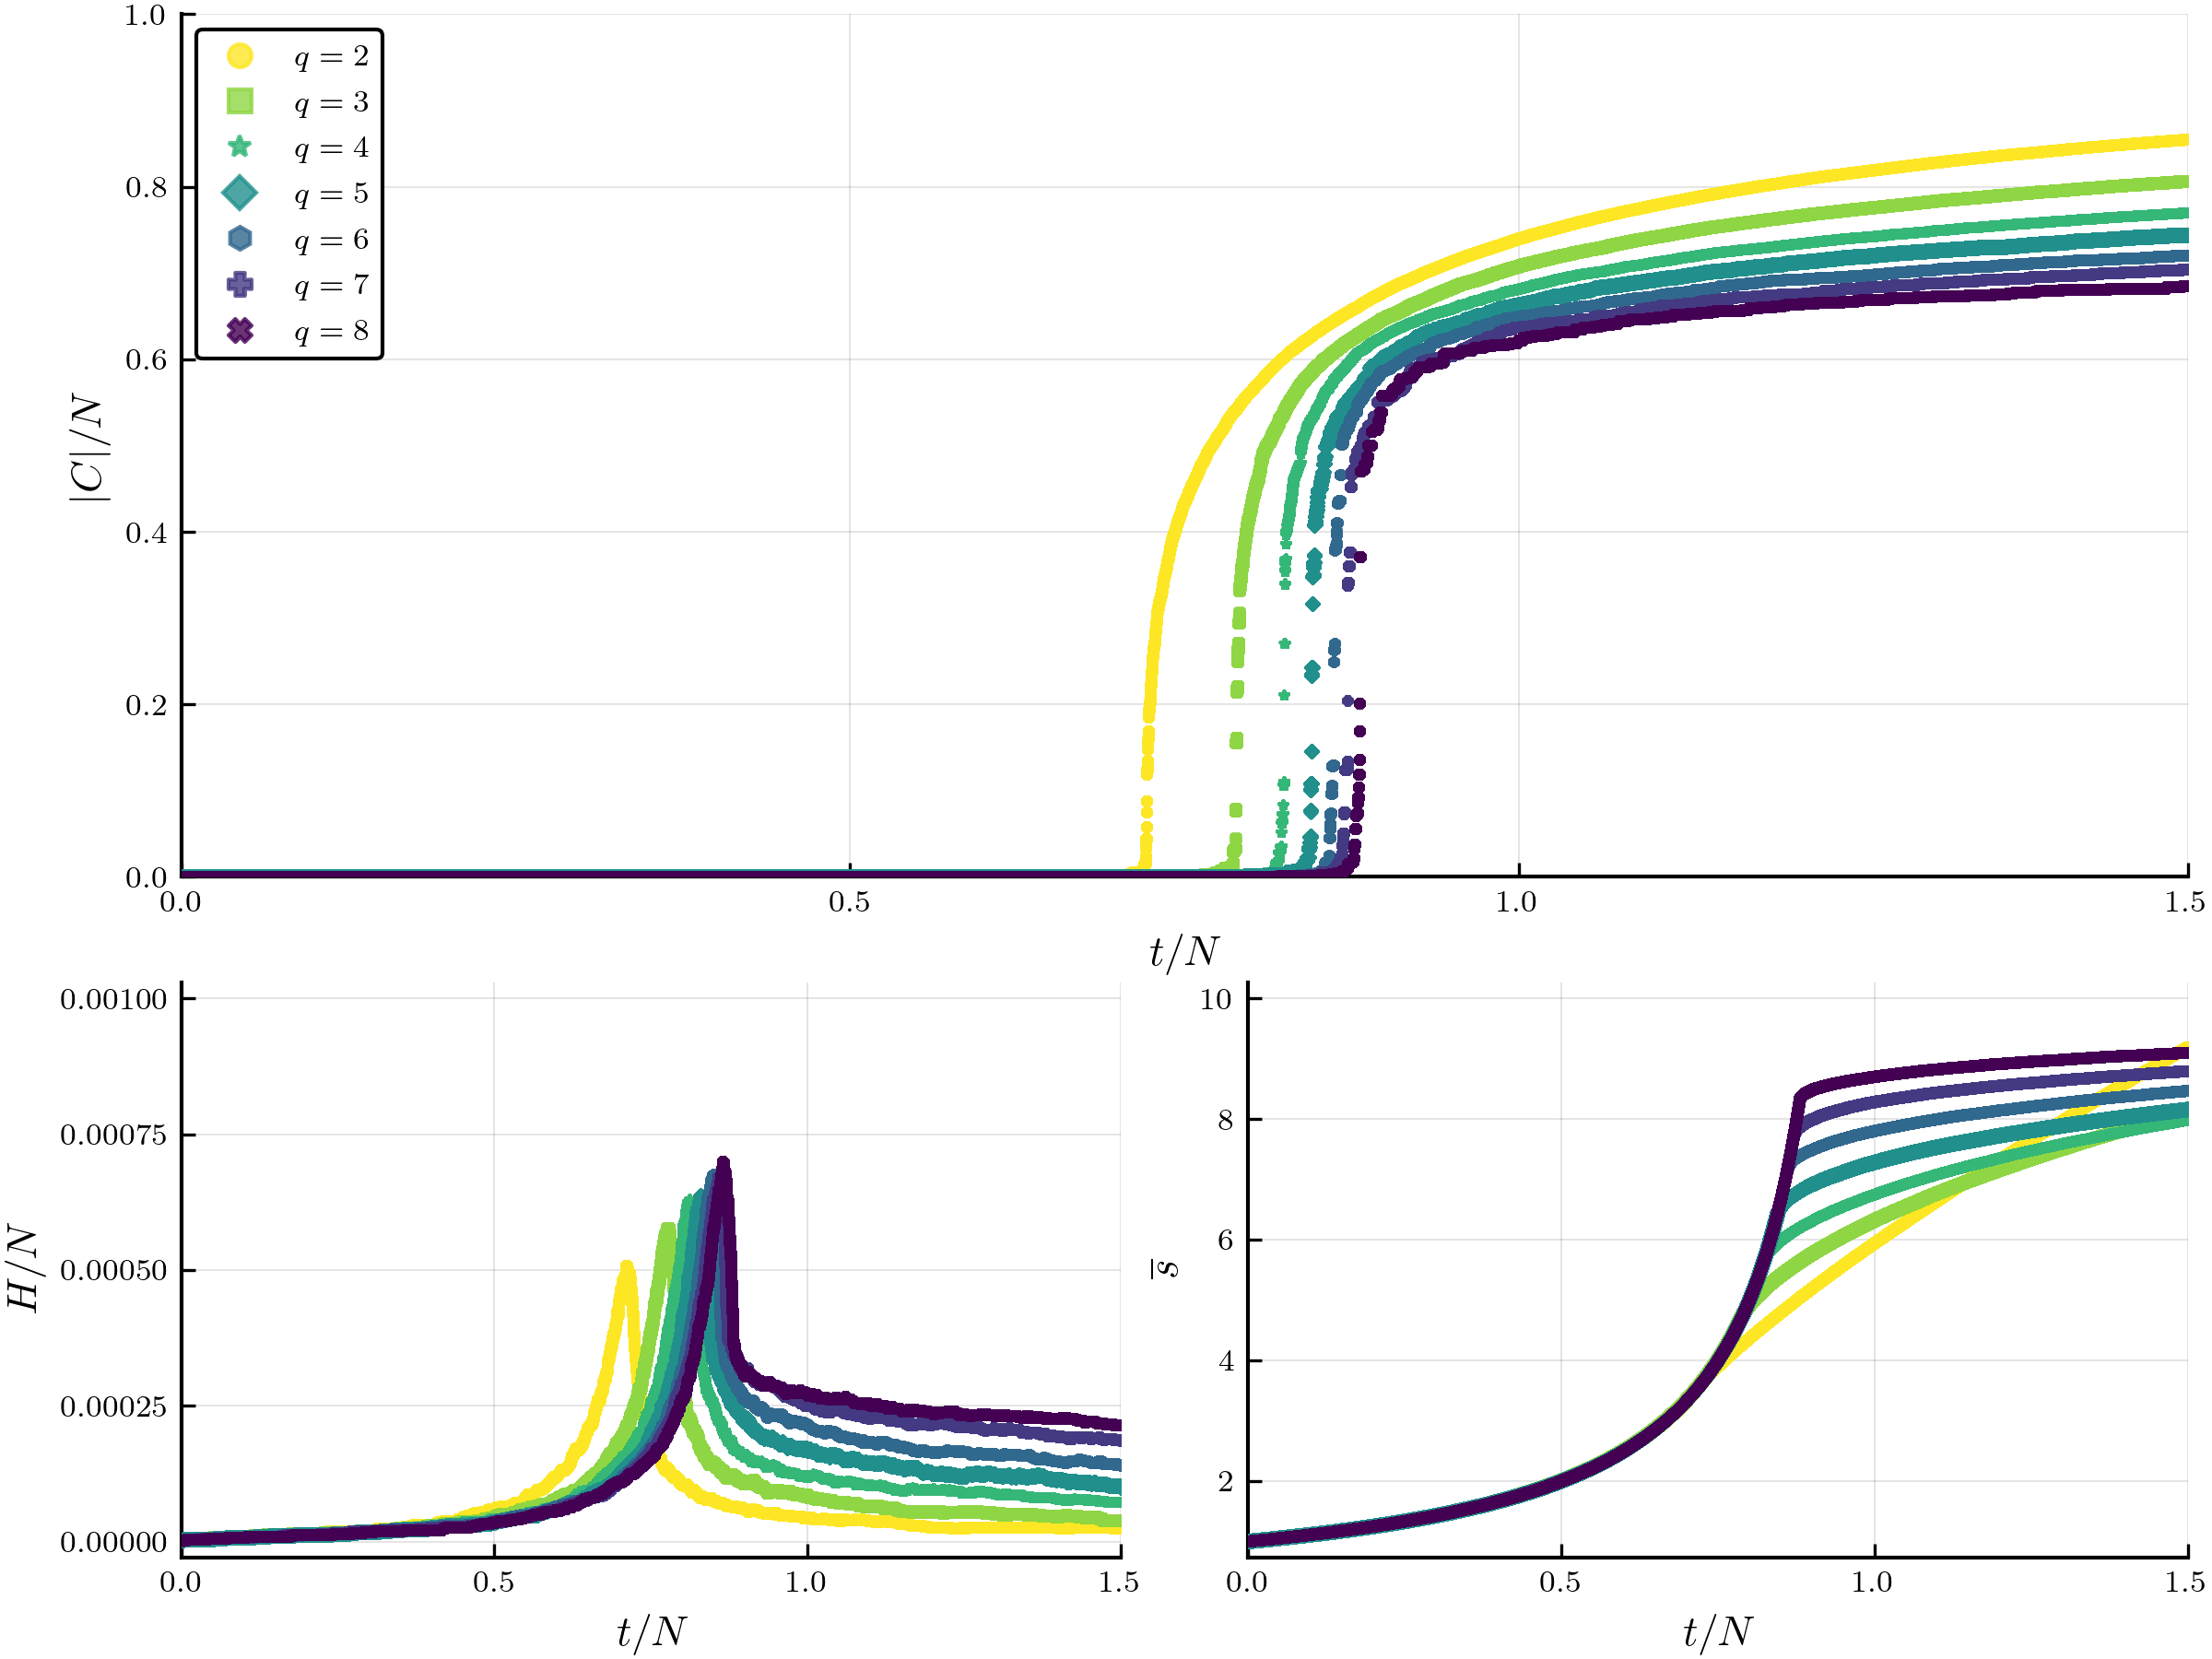
\includegraphics[width=350pt, clip]{images/q_scaling_triple.png}
	\caption{Stochastic edge acceptance model dependence on $q$. As $q$ increases we see the transition is delayed even longer. The heterogeneity per node exhibits sharper peaks, and the average cluster size shows interesting behavior. $N = 10^6$.}
	\label{fig:q_scaling_triple}
\end{figure}

Fig. \ref{fig:Lattice2D_ER_BF_PR_SEA_transition} illustrates what happens when we change the graph type to a 2D square lattice allowing only edges between nearest neighbors.
We see that doing so shifts order parameter to a later point, which makes sense due to the fact that on a two dimensional lattice each point only has four neighbors thus only four possible edges it can be connected with.

\begin{figure}[H]
	\centering
	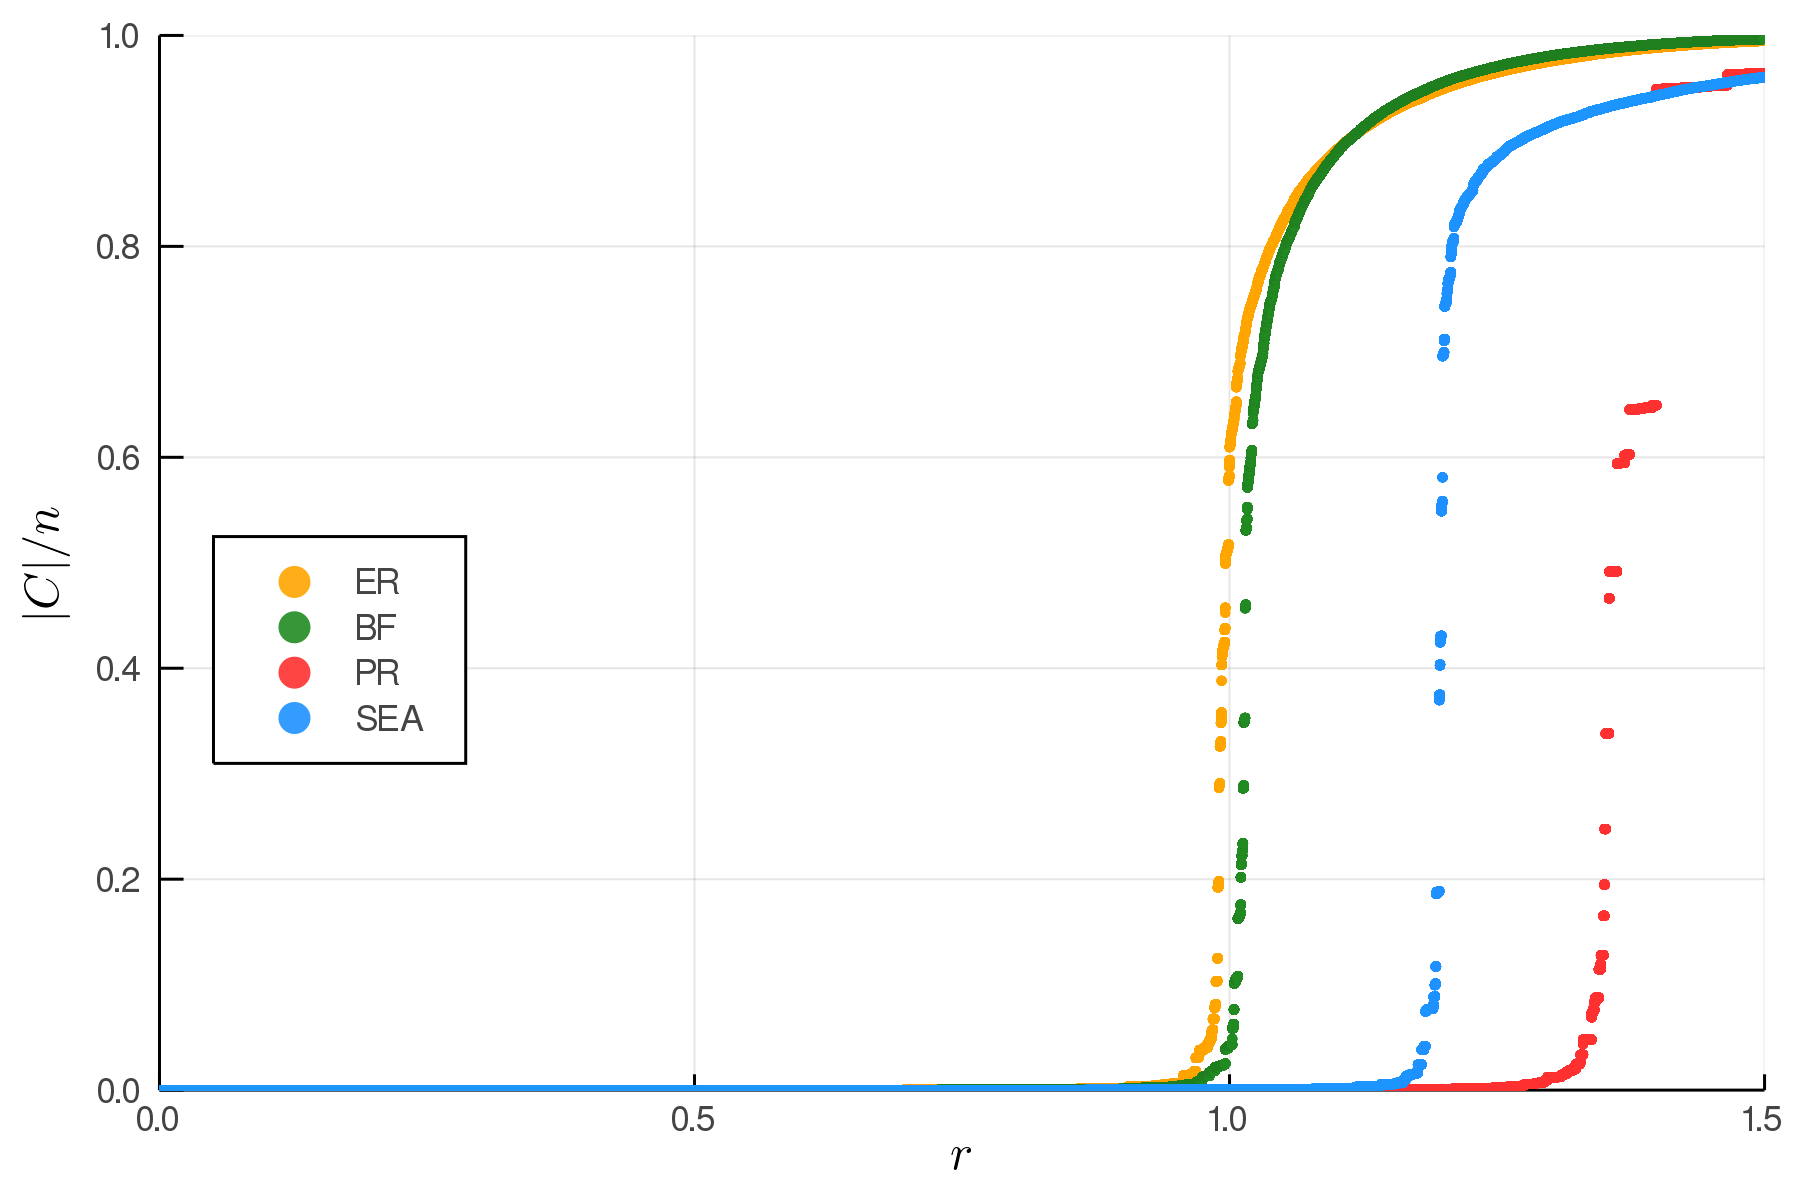
\includegraphics[width=350pt, clip]{images/Lattice2D_ER_BF_PR_SEA_1e6_order_param.png}
	\caption{Stochastic edge acceptance model order parameter when run on a 2D square lattice. $L = 10^3$.}
	\label{fig:Lattice2D_ER_BF_PR_SEA_transition}
\end{figure}

Fig. \ref{fig:Lattice3D_ER_BF_PR_SEA_transition} illustrates the case of allowing only nearest neighbor edges on a 3D cubic lattice. The transition is delayed longer than that in a random network but is before that on a 2D lattice, which again makes sense because now we have six neighbors with which we can activate edges between.

\begin{figure}[H]
	\centering
	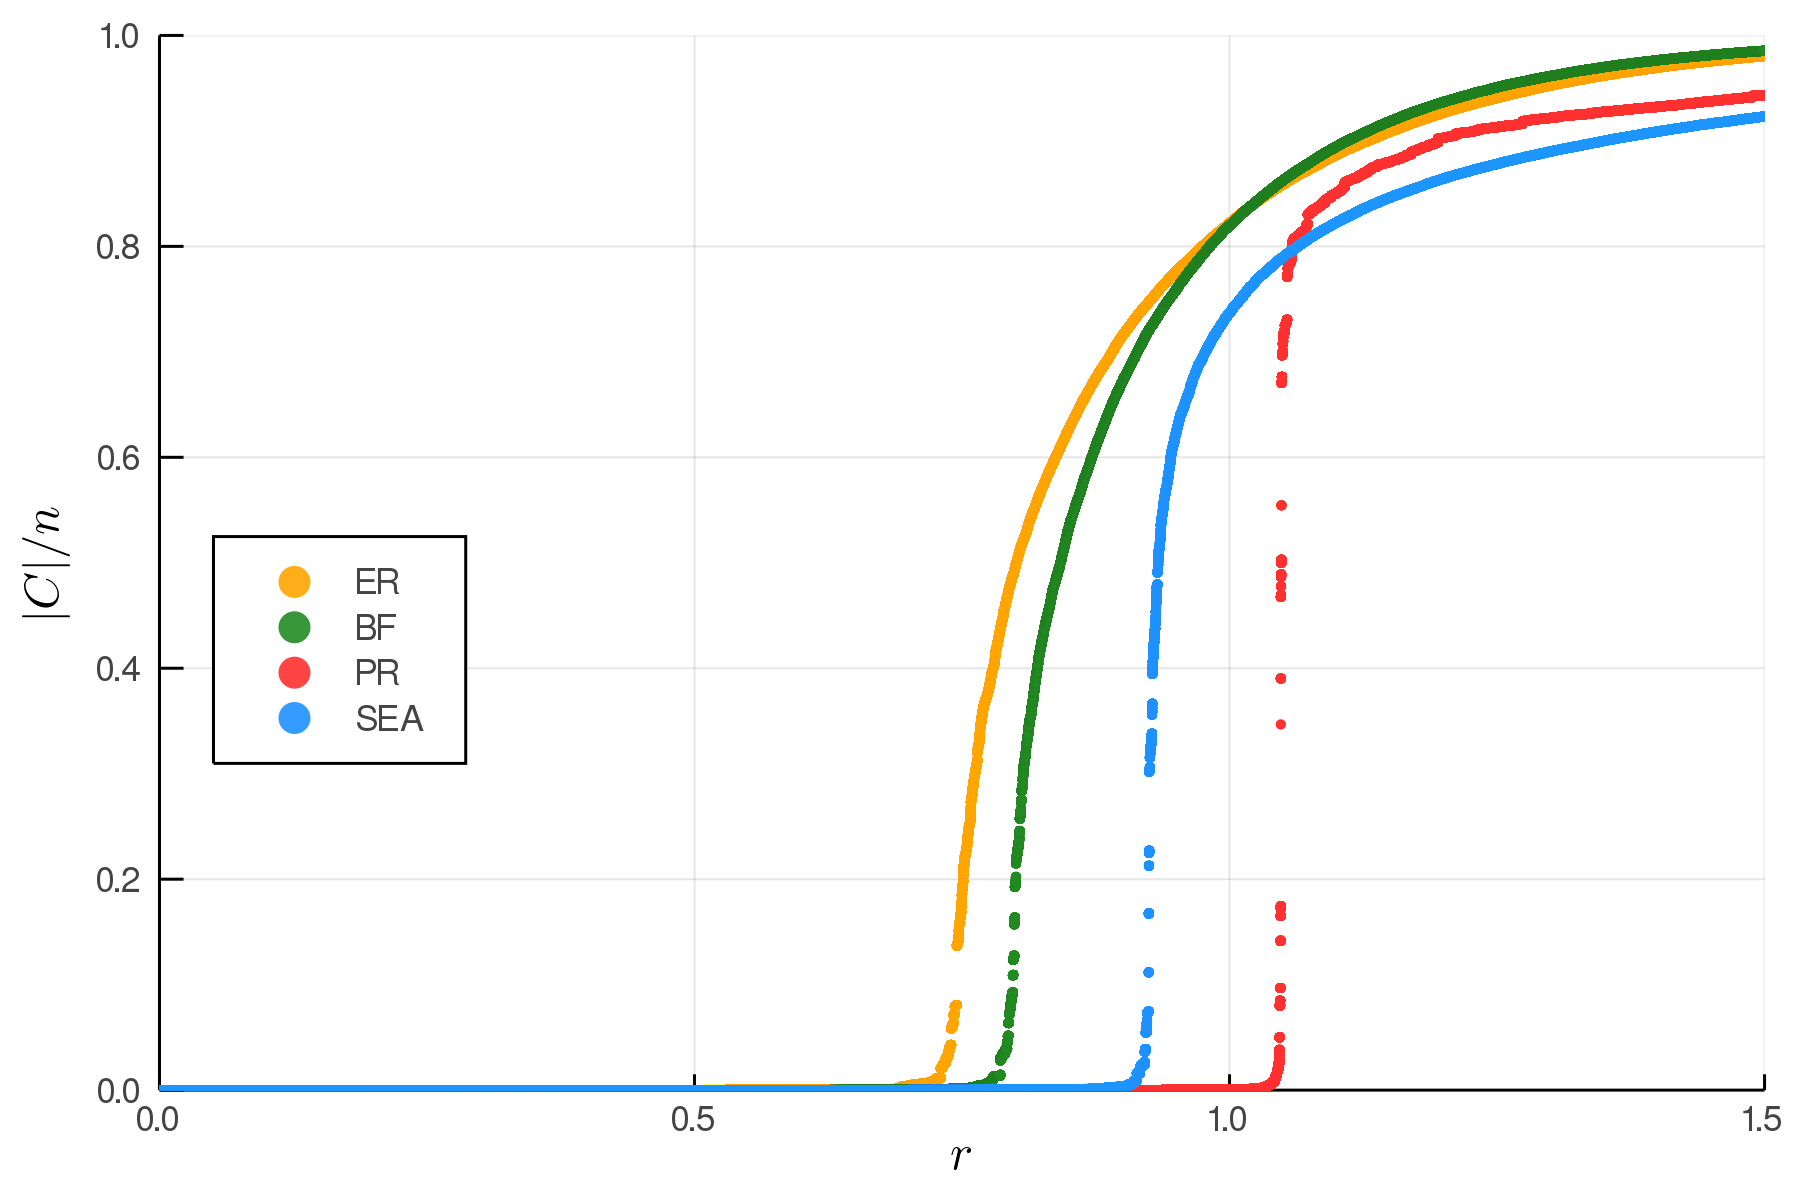
\includegraphics[width=350pt, clip]{images/Lattice3D_ER_BF_PR_SEA_1e6_order_param.png}
	\caption{Stochastic edge acceptance model order parameter when run on a 3D cubic lattice. $L = 10^2.$}
	\label{fig:Lattice3D_ER_BF_PR_SEA_transition}
\end{figure}


\chapter{Conclusion}
\label{ch:conclusion}
When Dmitris Achlioptas raised the question in 2000, he probably did not foresee the cascade of follow up questions it would lead to.
As we have seen, small changes to the way that edges are added to the graph can drastically alter the nature of the phase transition, leading up to what some people believe to be a discontinuous transition.
There was a lengthy debate over the course of several years discussing the continuity of these transitions, which as of now appears to have been resolved.
The deciding factor in whether or not these transitions are continuous is what information they take into account; algorithms that take only local information into account produce continuous transitions whereas some algorithms that take global information into account can product discontinuous transitions.

Since it was first discussed the topic of explosive percolation has been heavily researched and there have been many different models created and analyzed.
The product rule seems to be the most famous of them all, and is the rule which was initially believed to be discontinuous, but was later proved continuous after using more advanced analysis techniques combined with larger scale simulations.
The da Costa rule is another that was studied in depth, later leading to a full fledged theory on how to study such systems.
Even though these local information based models were proven continuous, they still show unusual finite-size scaling behavior and each are in their own universality class, which makes them interesting to study.

In \ref{ch:sea} we analyzed a new model (stochastic edge acceptance) using the framework laid out in \cite{Lee_1}, where we studied the scaling behavior of the cluster size distribution near the critical point to determine critical exponents which we used to place an upper bound on the order parameter, thus showing continuity.
The SEA model was merely a toy model to show proof of concept and to see how the phase transition would look like with a little extra randomness implemented.
Overall I think that the stochastic edge acceptance model was a success, as the data obtained from the simulations fit well with the framework within which we were studying it.

I believe that through this thesis I have gained a much deeper understanding of percolation theory and computational physics as a whole.
I very much enjoyed writing the associated library (GraphEvolve.jl) which I used to run my simulations, and it was extremely satisfying when the output data showed nice power law scaling relations near the critical point.
As of now I am happy with what I was able to accomplish here and the future directions listed at the end of Ch. \ref{ch:sea} are there and ready to be studied if I choose to dive further into this topic.

I must say thanks to Prof. Dr. Wolfhard Janke, Dr. Stefan Schnabel, M.Sc. Henrik Christiansen, and Alan Sammarone for the interesting and stimulating conversations regarding the topic of explosive percolation.


\appendix
\chapter{Appendix}
\label{ch:appendix}
\section{Designing the Library}
I chose Julia as the language to write the library in for several reasons, the largest being that I believe Julia is the perfect language for running large scale distributed computational physics/mathematics simulations.
The benefit of being able to use it as an interpreted language while at the same time getting speeds of a compiled language can not be understated since the immediate feedback and ability keep a kernel running with data in RAM allows for easy debugging and data exploration.
Julia code revolves around its type system which works nicely with its use of multiple dispatch, and at the heart of the type system is defining custom types and creating hierarchies with which functions can take specific types.
The type hierarchy of Julia's default types is illustrated in Fig. \ref{fig:julia_type_hierarchy}.

\begin{figure}[H]
	\centering
	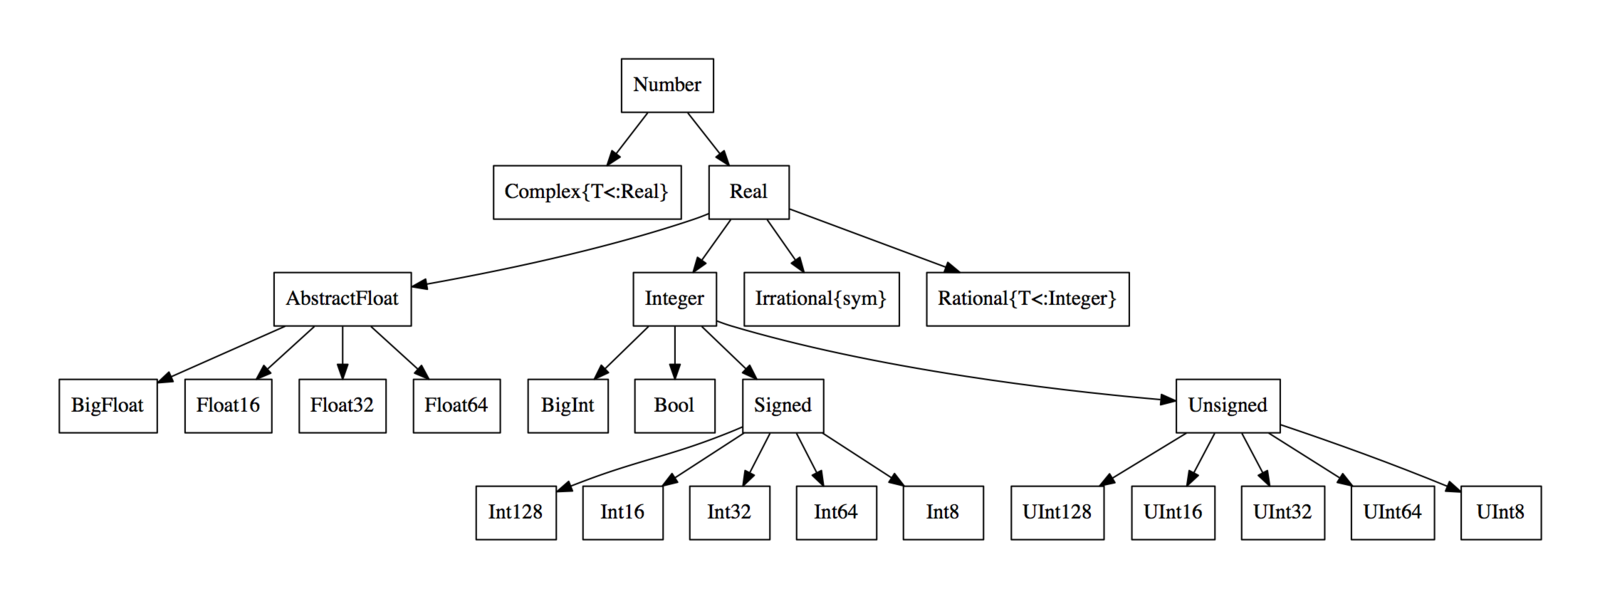
\includegraphics[width=400pt]{images/julia_type_hierarchy.png}
	\caption{Julia Type Hierarchy}
	\label{fig:julia_type_hierarchy}
\end{figure}

The type system is actually opt-in, meaning that one need not type their variables, but typing can help with performance as well as gaining a better understanding of how the code works.

I started off with creating custom types to represent networks/lattices, the type hierarchy of them is illustrated below in Fig. \ref{fig:custom_type_hierarchy}.

\begin{figure}[H]
	\centering
	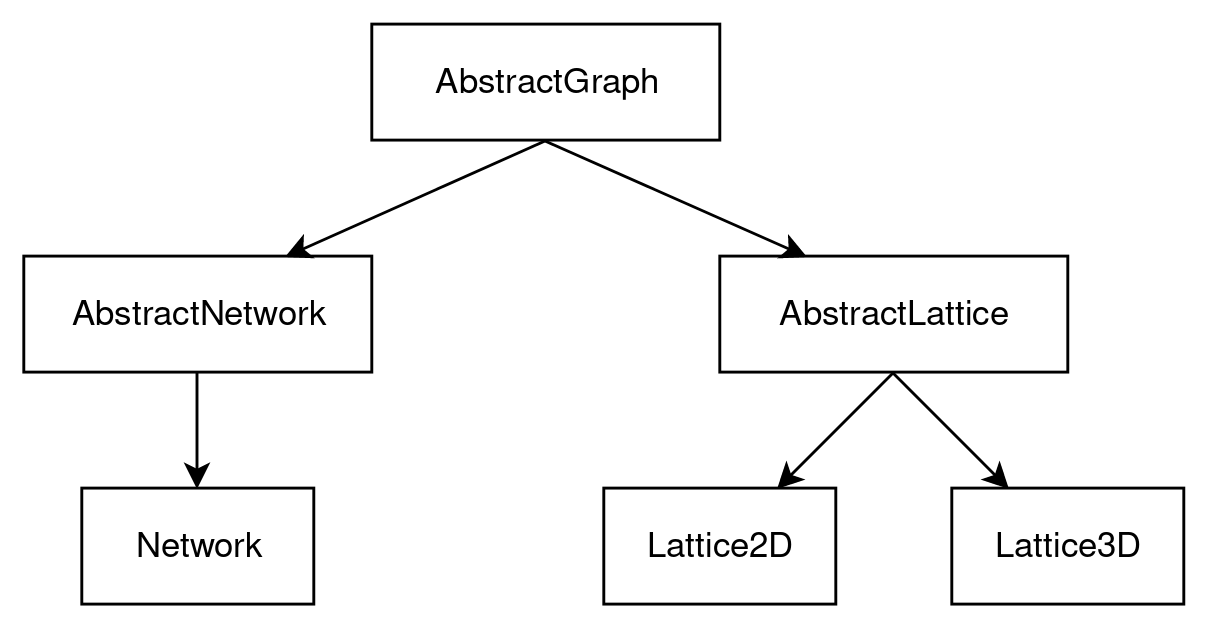
\includegraphics[width=350pt]{images/custom_type_hierarchy.png}
	\caption{Custom Type Hierarchy}
	\label{fig:custom_type_hierarchy}
\end{figure}

As of now there are three different types of graphs: \texttt{Network}, \texttt{Lattice2D}, and \texttt{Lattice3D}.
The \texttt{Network} type represents an undirected network where edges can be present between any two unique nodes.
The \texttt{Lattice2D} type represents a two-dimensional square lattice where edges can be present only between nearest neighbors, similarly where \texttt{Lattice3D} represents a three-dimensional cubic lattice.
The following is a brief conceptual overview of how the system functions, for more detailed descriptions and explanations of methods or variables please refer to the documentation.

Each of these types have a similar structure in the way they store information about the underlying graph they represent.
To instantiate a type one must pass it the size and optionally a seed value for the random number generator (which is used in the evolution for randomly selecting edges), which in a \texttt{Network} means passing the number of nodes \texttt{n} and in a \texttt{LatticedD} passing the side length \texttt{L} ($\texttt{n} = \texttt{L}^\texttt{d}$).
The types also have a variable called \texttt{t} which refers to the step in the evolution process and represents the number of edges present in the graph.
The edges present in the graph are kept track in the \texttt{edges} variable, which is a set of two-tuples of integers representing an edge between node \texttt{i} and \texttt{j} as \texttt{(i, j)}.
As of now the edges in all types are undirected i.e. \texttt{(i, j) = (j, i)}, but only \texttt{(i, j)} is stored to minimize unnecessary RAM usage.

Keeping track of the clusters as they evolve is the meat of these simulations, therefore it is necessary to speak about how this is done.
\texttt{cluster\_ids} is a \texttt{d}-dimensional array \texttt{(d = 1 (Network), 2 (Lattice2D), 3 (Lattice3D))} which contains the information relating to which cluster a node is in.
\texttt{clusters} is a dictionary where the keys are the cluster IDs and the values are sets of nodes which are in the given cluster.
\texttt{cluster\_sizes} is a dictionary where the the keys are the cluster IDs and the values are integers representing the number of nodes in the given cluster.
The associated observables are stored in a custom type called \texttt{Observables} under the name \texttt{observables}.

Now that we understand how the clusters are tracked let's talk about how this is done in reality.
Let \texttt{t} be the current step in the evolution process where edge \texttt{(i, j)} has been chosen to be added to the graph.
Let $C_\texttt{i}$ represent the cluster to which node \texttt{i} is a member of, i.e. $\texttt{i} \in C_\texttt{i}$.
We then look and determine which cluster is smaller and merge the smaller cluster into the larger cluster in-place (this small trick saves a significant amount of computational time), e.g. if $|C_\texttt{j}| < |C_\texttt{i}|$ then all of the nodes in $C_\texttt{j}$ will have their cluster ID updated to that of $C_\texttt{i}$ and the set of nodes representing $C_\texttt{i}$ will be updated to include the nodes in $C_\texttt{j}$, and the entry for $C_\texttt{j}$ will then be deleted from \texttt{clusters} to reduce the memory footprint.

After the clusters are merged the associated observables are updated, which currently includes the largest cluster size, the average cluster size, the cluster heterogeneity (number of unique cluster sizes), and some post-simulation analysis quantities for identifying where the phase transitions and if it is continuous.

\subsection{Making Use of Multiple Dispatch}
Multiple dispatch allows us to define multiple functions with the same name, yet different code depending on the input type.
This is extremely useful for dealing with differences between networks and lattices such as when selecting an edge, because for example in a \texttt{Network} we can select any inactive edge between nodes, whereas in a \texttt{LatticedD} we can only select an inactive edge between nearest neighbors (this can be seen implemented in \texttt{edge\_methods.jl}).

Another benefit of this coupled with the type system is that when we have a function that is generic enough to act on both \texttt{Network}s and \texttt{LatticedD}s then we can set the input type for that function to \texttt{AbstractGraph} or if it's general enough to act on all \texttt{LatticedD}s but not \texttt{Network}s then we can set the input type to \texttt{AbstractLattice}.
This allows for consistency, e.g. we can call \texttt{product\_rule!(Network(Int(1e6)))} and similarly \texttt{product\_rule!(Lattice2D(Int(1e3)))} and the code will decide based on the type which functions to use.

\subsection{Running a Simulation}
Running a simulation is simple, one must first download the \texttt{Percolation.jl} library, which can be found on GitHub under the MIT license.
Then, to run a simulation on a \texttt{Network} with $10^6$ nodes using the product rule to add $1.5 \cdot 10^6$ edges, and view the largest cluster size time series data we would run:

\begin{lstlisting}
# add the library to the load path and import it
push!(LOAD_PATH, "/path/to/Percolation.jl/src")
using Percolation

# instantiate the Network
g = Network(Int(1e6))

# run the evolution process
product_rule!(g, Int(1.5e6))

# show the largest cluster size time series data
g.observables.largest_cluster_size
\end{lstlisting}


\printbibliography

\end{document}
